\section{Estimation of the Standard Model Backgrounds}
\label{sec:stop_background_estimate}

In this section, we describe the methods used for the estimation of the SM background
contamination in the SRs.
By Table~\ref{tab:stop_exp_sr_yield}, it can be seen that the expected SM background
contamination to the SRs in the \bWN search is primarily composed of events
from the \ttbar~and diboson processes.
Given that these are the dominant backgrounds for the analysis, their estimation is performed
using the control region method, described in Section~\ref{sec:control_region_method}.
That is, dedicated CRs and VRs are defined for each of the two processes in order
to provide a normalisation correction for their MC prediction in the SRs.
All other background processes, being subdominant, have their predicted contribution
to the SR background taken directly from the MC simulation.
The estimation of the contribution of sources leading to fake and non-prompt leptons
is performed using the Matrix Method, described in Section~\ref{sec:matrix_method}.

Sections~\ref{sec:stop_ttbar_estimate} and \ref{sec:stop_vv_estimate} describe
the background estimate for the \ttbar~and diboson processes, respectively.

The CR and VR definitions for both the \ttbar~and diboson background are based on the
SR definitions given in the previous section.
The CRs are defined primarily by inverting the two-dimensional selection
made in the $(\cosb, \dpb)$-plane, and maintaining similar selections as in the SRs for the other variables.
The VRs, on the other hand, are defined by inverting the selections on the non-angular variables relative to those
made in the SRs.

\begin{figure}[!htb]
    \begin{center}
        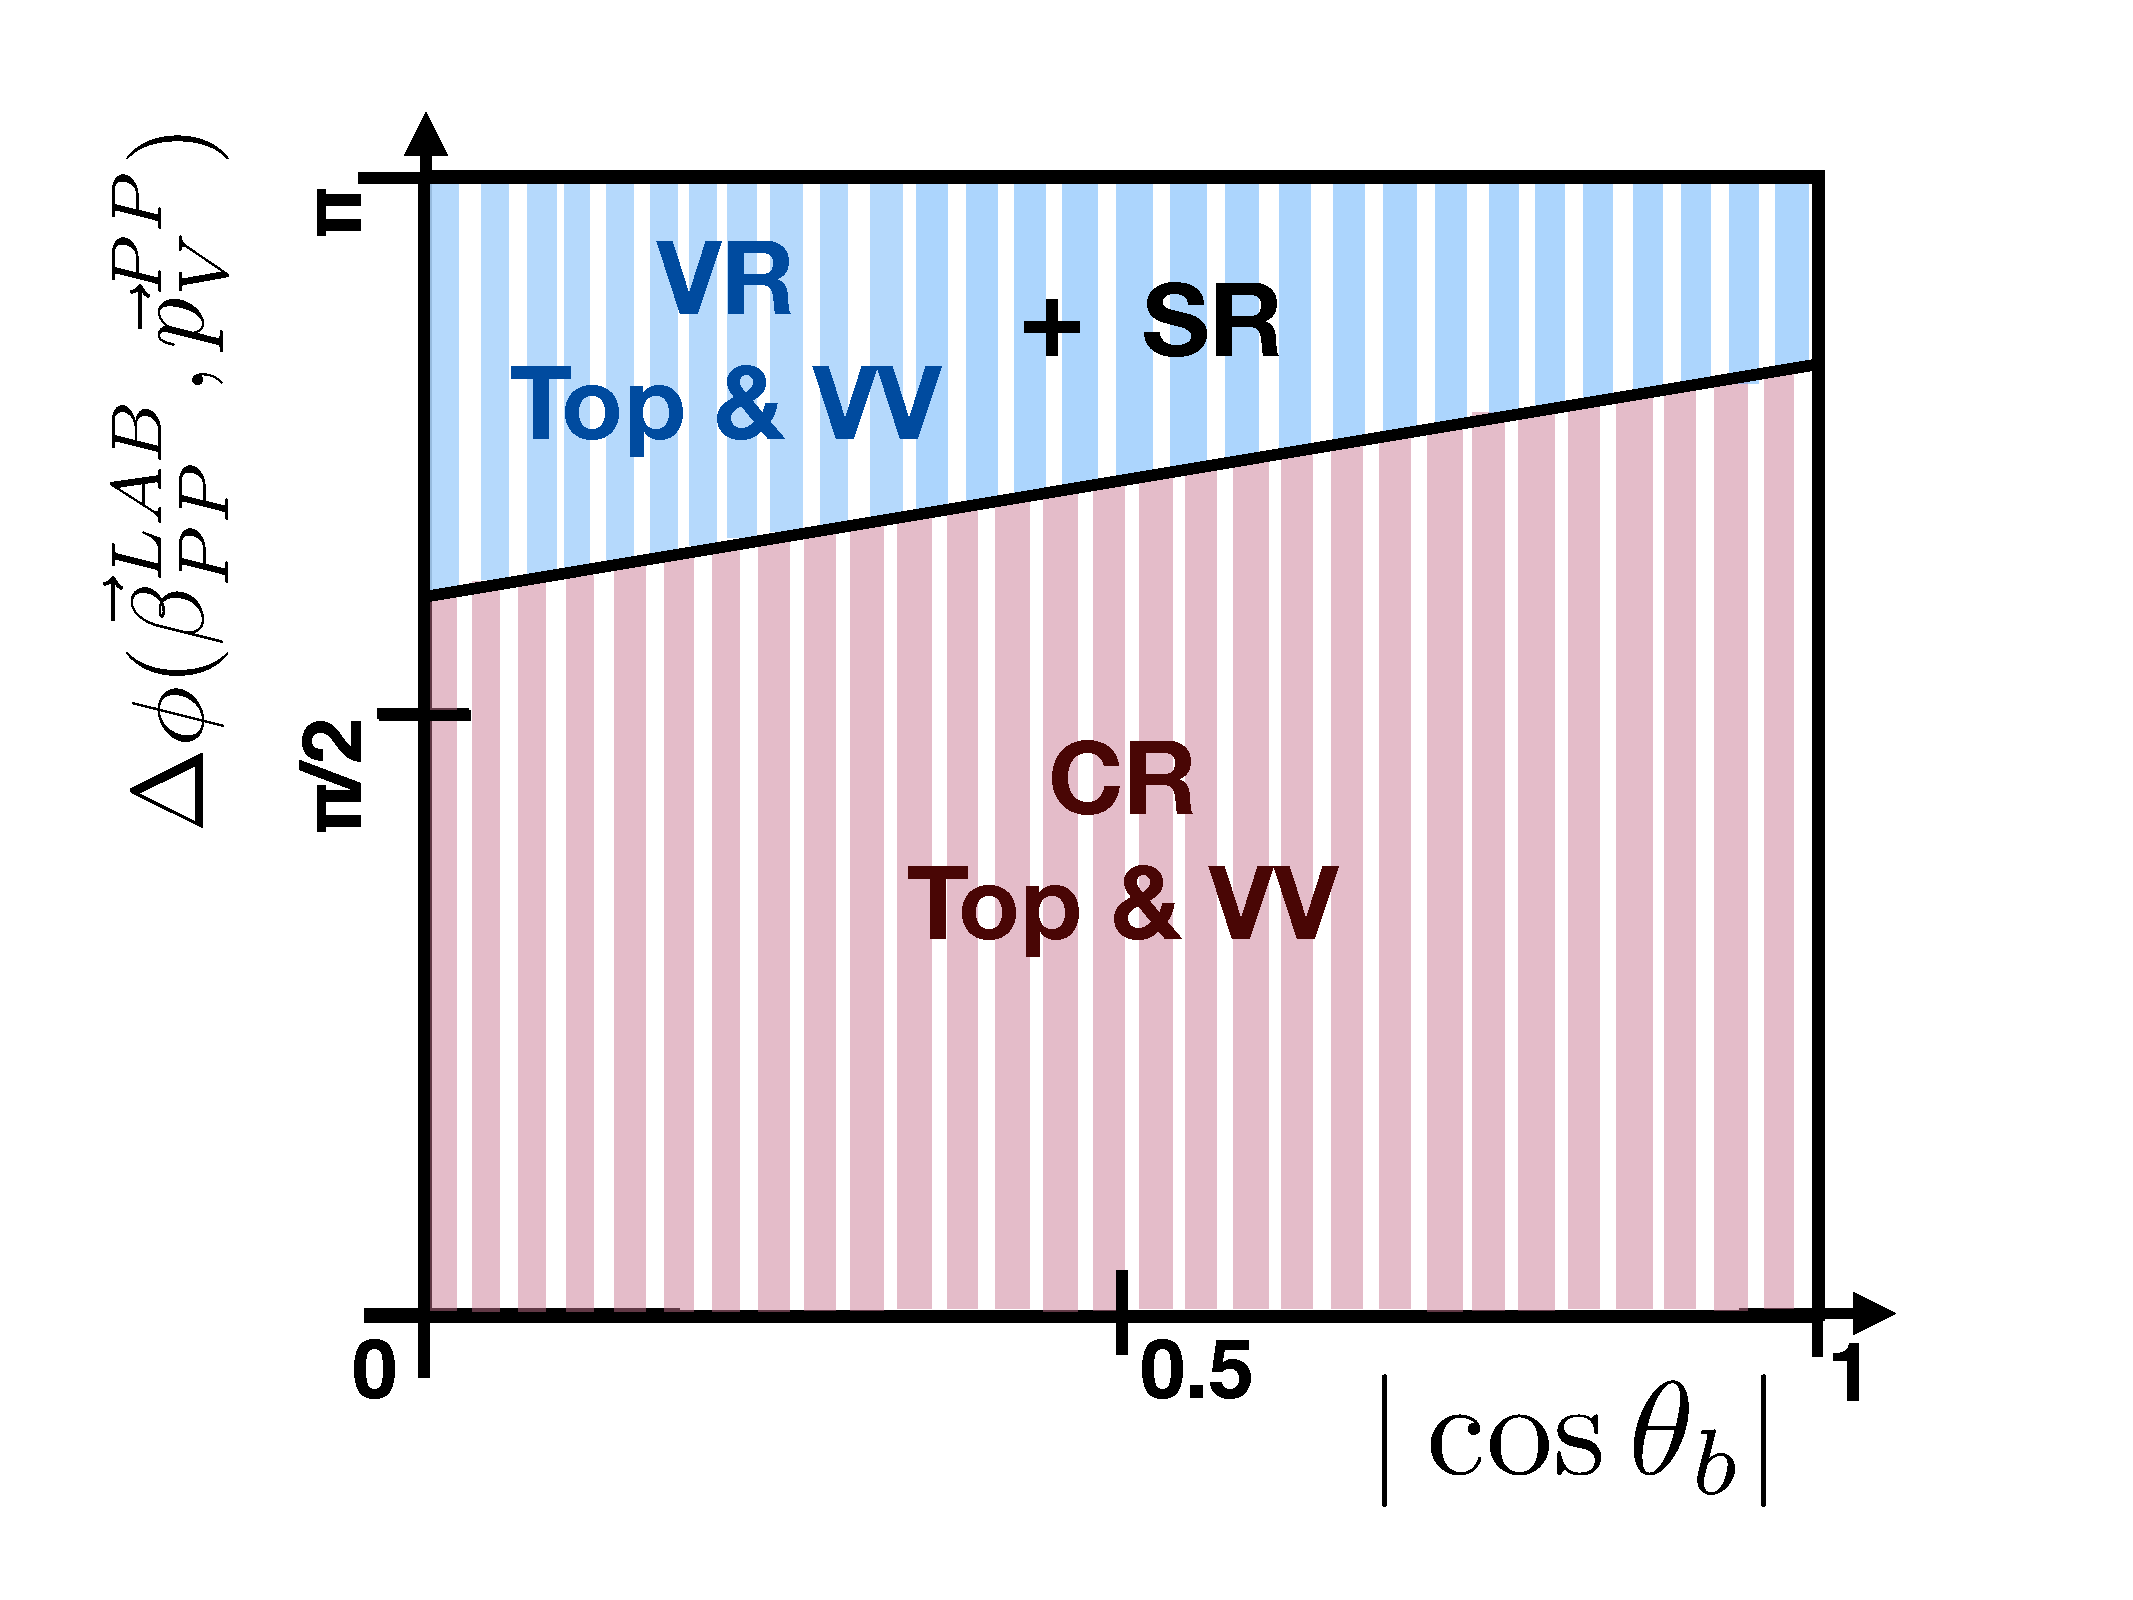
\includegraphics[width=0.7\textwidth]{figures/search_stop2l/bkg_est/crvrmotivation}
        \caption{
            Illustration of the CR and VR strategy used in the \bWN search.
            The defining characteristic for the definition of these regions is
            based on the region in the $(\cosb, \dpb)$-plane that they select.
            The CR inverts the requirements on these quantities relative to the SRs,
            while the VR has the same requirements as in the SRs but inverts
            selections made on the other observables.
        }
        \label{fig:stop_crvr_motivation}
    \end{center}
\end{figure}

\FloatBarrier
%%%%%%%%%%%%%%%%%%%%%%%%%%%%%%%%%%%%%%%%%%%%%%%%%%%%%%%%%%%%%%%%%%%%%%%%%%%%%%%%%%%%%%%%%%%%
%%%%%%%%%%%%%%%%%%%%%%%%%%%%%%%%%%%%%%%%%%%%%%%%%%%%%%%%%%%%%%%%%%%%%%%%%%%%%%%%%%%%%%%%%%%%
%%%%%%%%%%%%%%%%%%%%%%%%%%%%%%%%%%%%%%%%%%%%%%%%%%%%%%%%%%%%%%%%%%%%%%%%%%%%%%%%%%%%%%%%%%%%
%
% TOP BKG
%
%%%%%%%%%%%%%%%%%%%%%%%%%%%%%%%%%%%%%%%%%%%%%%%%%%%%%%%%%%%%%%%%%%%%%%%%%%%%%%%%%%%%%%%%%%%%
%%%%%%%%%%%%%%%%%%%%%%%%%%%%%%%%%%%%%%%%%%%%%%%%%%%%%%%%%%%%%%%%%%%%%%%%%%%%%%%%%%%%%%%%%%%%
%%%%%%%%%%%%%%%%%%%%%%%%%%%%%%%%%%%%%%%%%%%%%%%%%%%%%%%%%%%%%%%%%%%%%%%%%%%%%%%%%%%%%%%%%%%%

\subsection{Top-quark pair production}
\label{sec:stop_ttbar_estimate}

The CRs and VRs designed to derive and validate the semi-data-driven
normalisation correction factor for the \ttbar~background process are called
CR-Top and VR-Top, respectively, and are defined in Table~\ref{tab:stop_top_crvr}.
The strategy for the CR and VR selections in the $(\cosb, \dpb)$ plane are described
in the previous section.
Several of the selections on the kinematic quantities relative to those in the SRs (c.f. Table~\ref{tab:stop_sr_def})
are relaxed.
In both CR-Top and VR-Top, the \mdr requirement is relaxed to $\mdr > 80$\,GeV and the requirement on the
\gaminv quantity is removed.
In VR-Top, the \rpt requirement is inverted relative to that used in the SRs.
Given that the \ttbar~background is flavor symmetric, only different-flavor events
are allowed to populate CR-Top and VR-Top, in order to avoid contamination from $Z$-boson processes.
As a result, no additional requirement on $m_{\ell\ell}$ is made in these regions.
For increased purity, CR-Top requires that there be at least one $b$-tagged jet,
while VR-Top applies a veto in order to be orthogonal to CR-Top.

VR-Top is defined to have zero $b$-tagged jets, while CR-Top requires at least one.
In dedicated studies, it has been verified that the \ttbar~normalisation correction derived
in the $b$-jet rich region CR-Top is well extrapolated to separate validation regions, and is rather
independent of the $b$-tagged jet multiplicity.
This gives confidence that VR-Top can be used as an appropriate check on the \ttbar~normalisation
correct factor and that it's extrapolation to the SRs, which have differing requirements on the
$b$-tagged jet multiplicity, is reasonable.

Distributions of several key observables in CR-Top are shown in Figures~\ref{fig:crt_0}-\ref{fig:crt_1}.

\begin{table}[!htb]
    \begin{center}
        \begin{scriptsize}
        \caption{
            Definitions of the CR and VR for the \ttbar~background process for the
            \bWN search.
        }
        \label{tab:stop_top_crvr}
        \begin{tabular}{l | c c}
            \hline
            \hline
                & \multicolumn{2}{c}{\textbf{Regions}} \\
            \hline
            \textbf{Variable} & \textbf{CR-Top} & \textbf{VR-Top} \\
            \hline
            Dilepton Flavor & DF & DF \\
            $m_{\ell\ell}$ [GeV]    & no req. & no req. \\
            Lead lepton \pT~[GeV] & $>25$ & $>25$ \\
            Sub-lead lepton \pT~[GeV] & $>20$ & $>20$ \\
            $b$-tagged jet multiplicity & $>0$ & Exactly 0 \\
            \mdr [GeV] & $>80$ & $>80$ \\
            \rpt & $>0.7$ & $<0.7$ \\
            \gaminv & no req. & no req. \\
            $(\cosb, \dpb)$ & \multicolumn{1}{c}{\small{$\dpb < 0.9 \times | \cosb | + 1.6$}} & \multicolumn{1}{c}{\small{$\dpb> 0.9 \times | \cosb | + 1.6$}} \\
            \hline
            \hline
        \end{tabular}
        \end{scriptsize}
    \end{center}
\end{table}

\subsubsection{Kinematic Distributions in CR-Top}

\begin{figure}[!htb]
    \begin{center}
        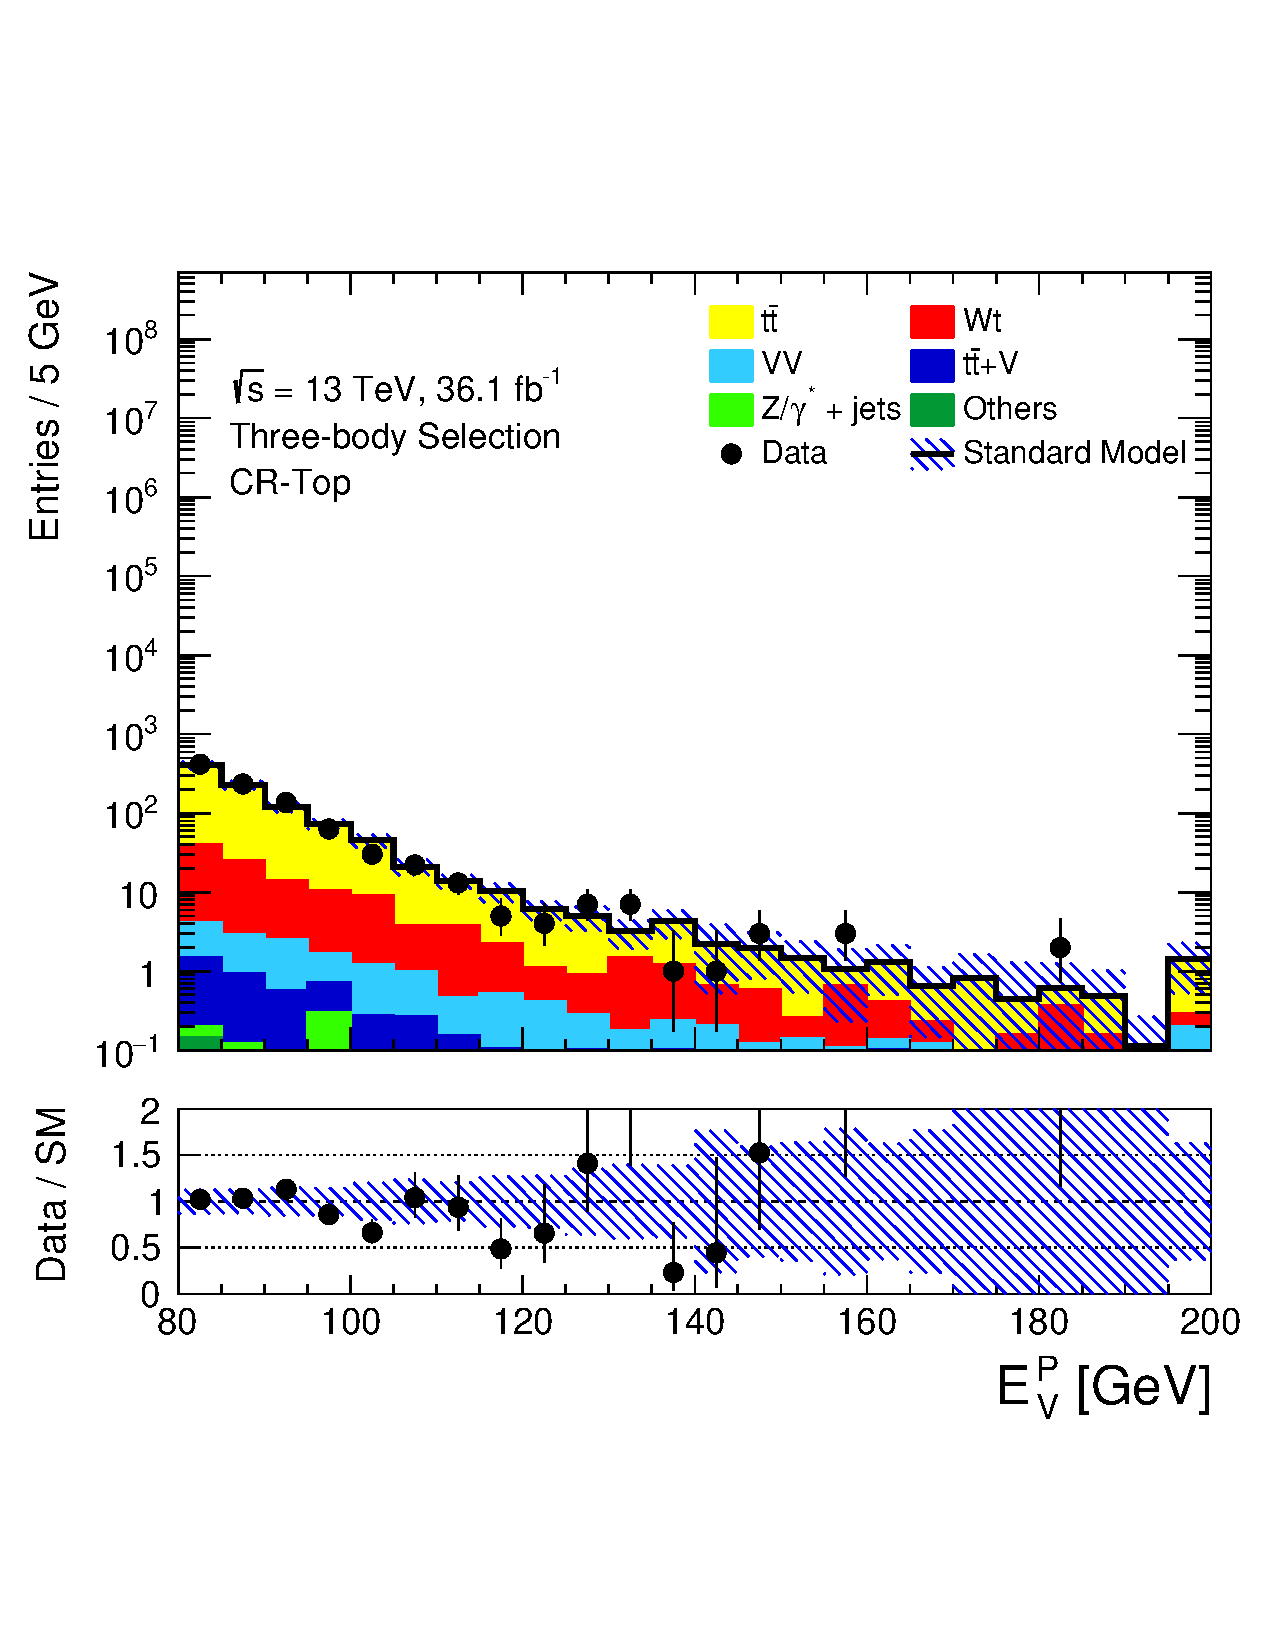
\includegraphics[width=0.48\textwidth]{figures/search_stop2l/bkg_est/crtop/crt_MDR}
        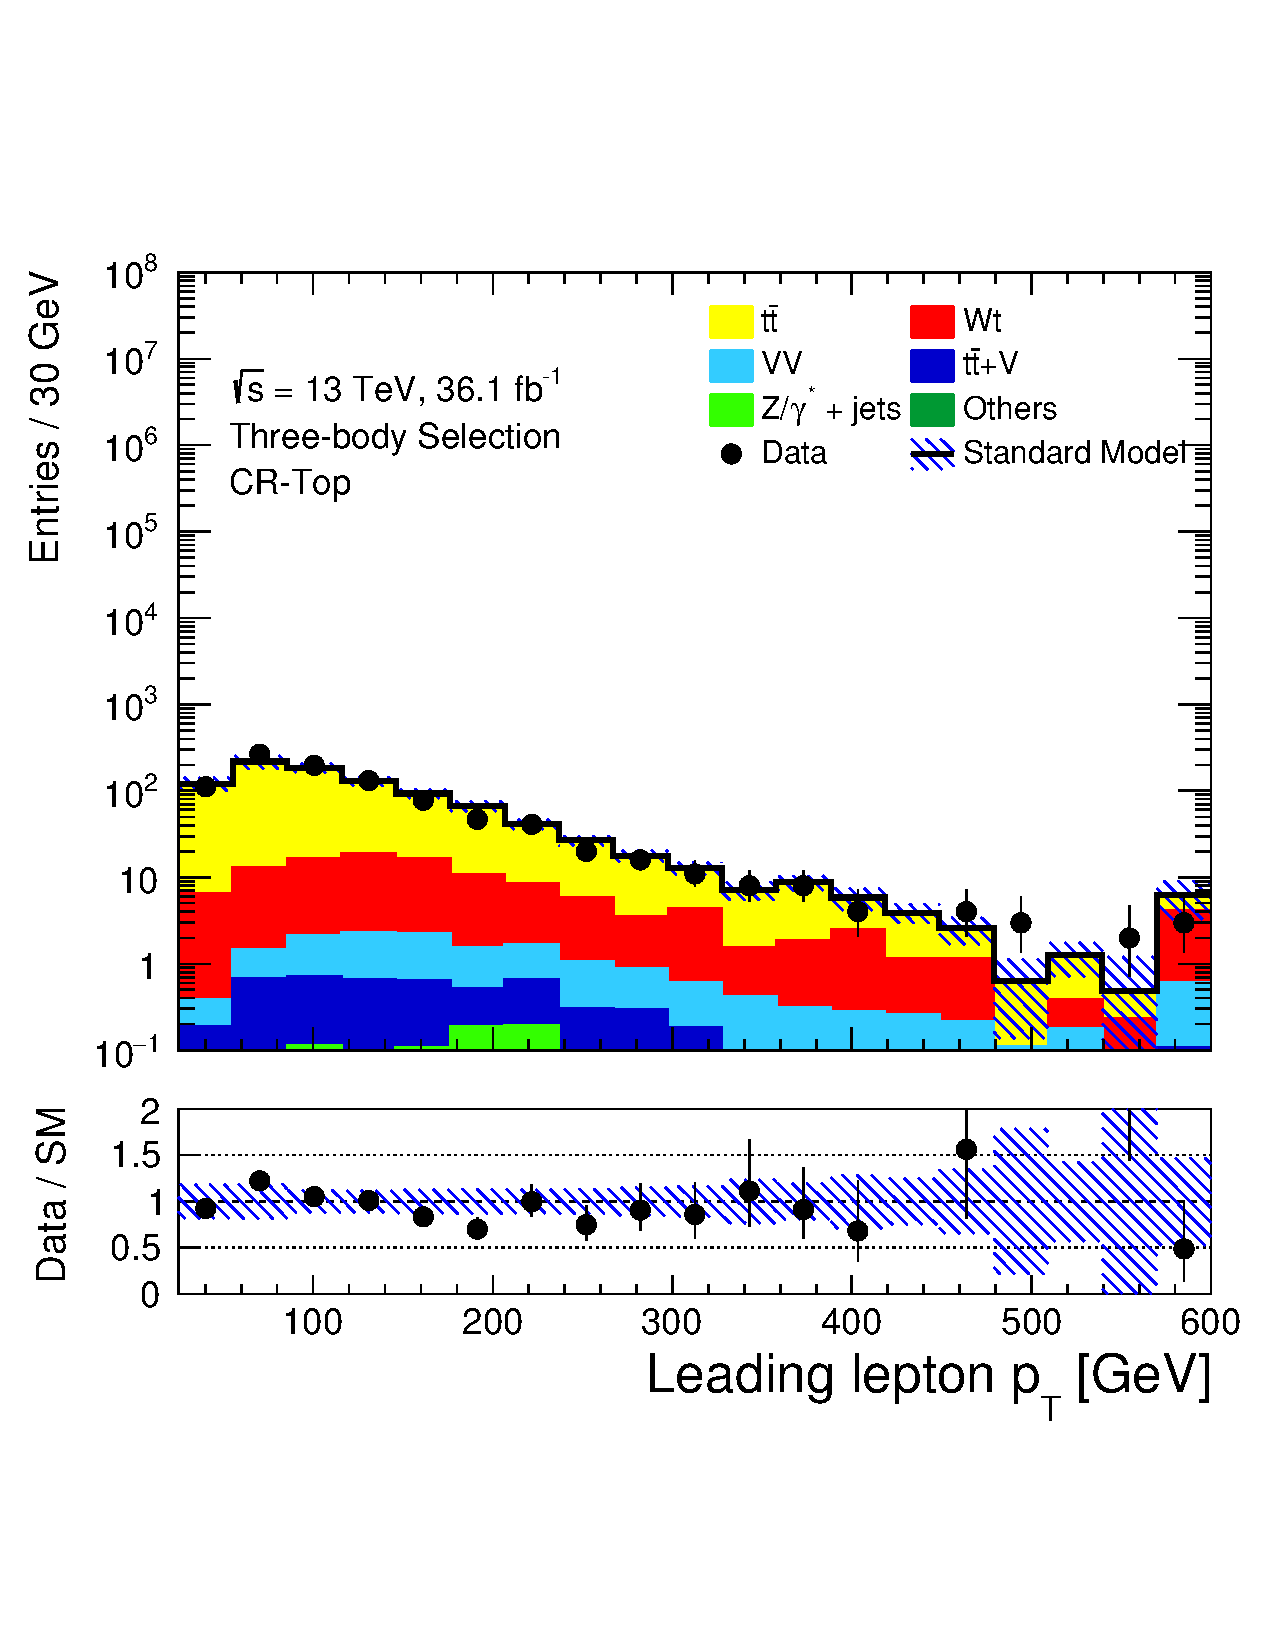
\includegraphics[width=0.48\textwidth]{figures/search_stop2l/bkg_est/crtop/crt_l_pt0}
        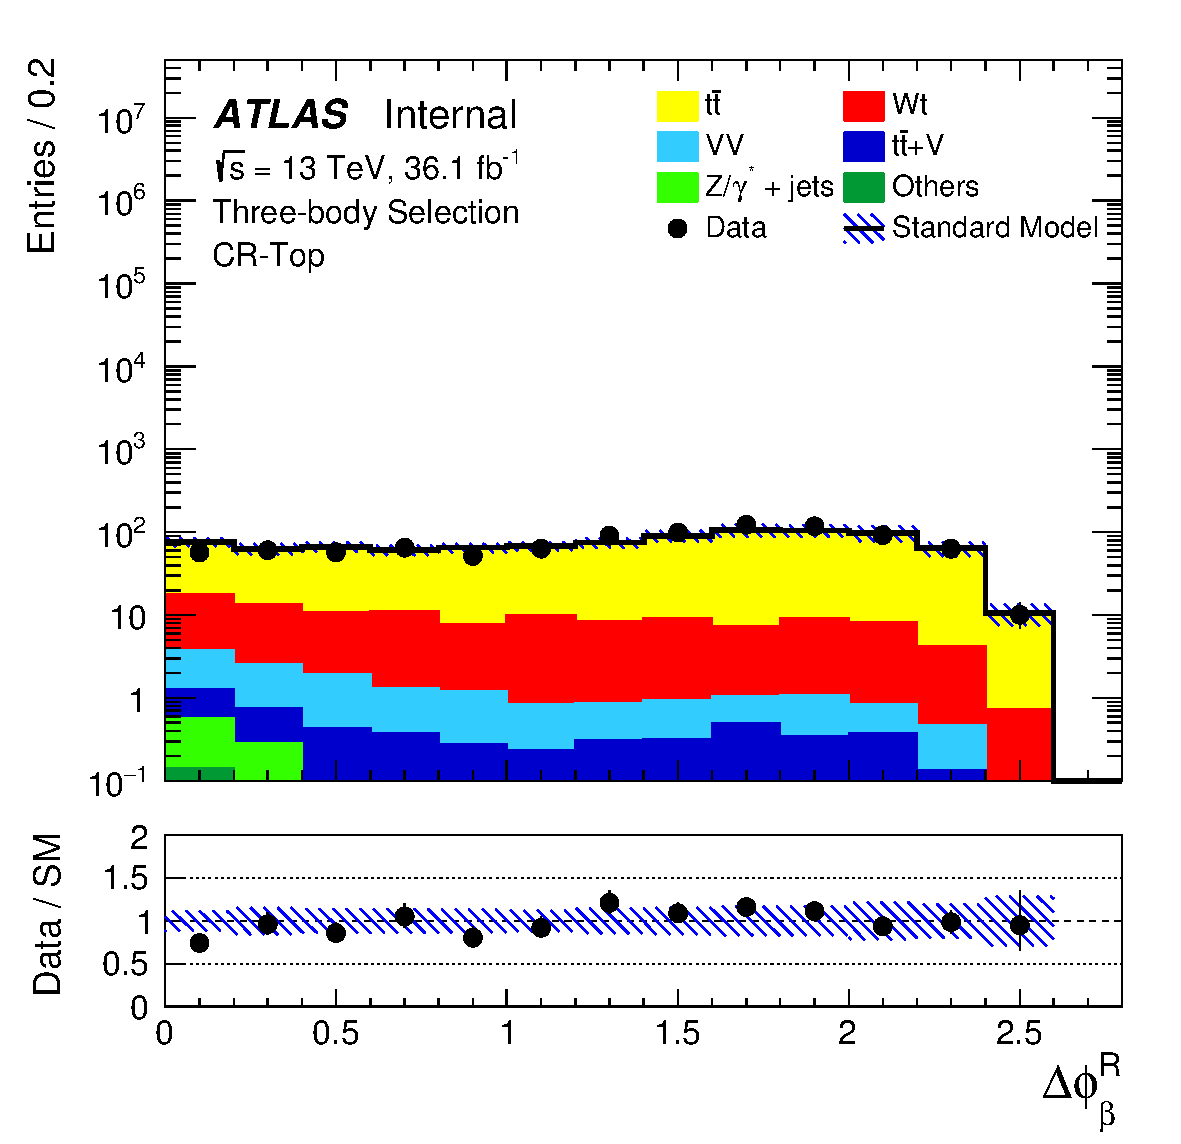
\includegraphics[width=0.48\textwidth]{figures/search_stop2l/bkg_est/crtop/crt_DPB_vSS}
        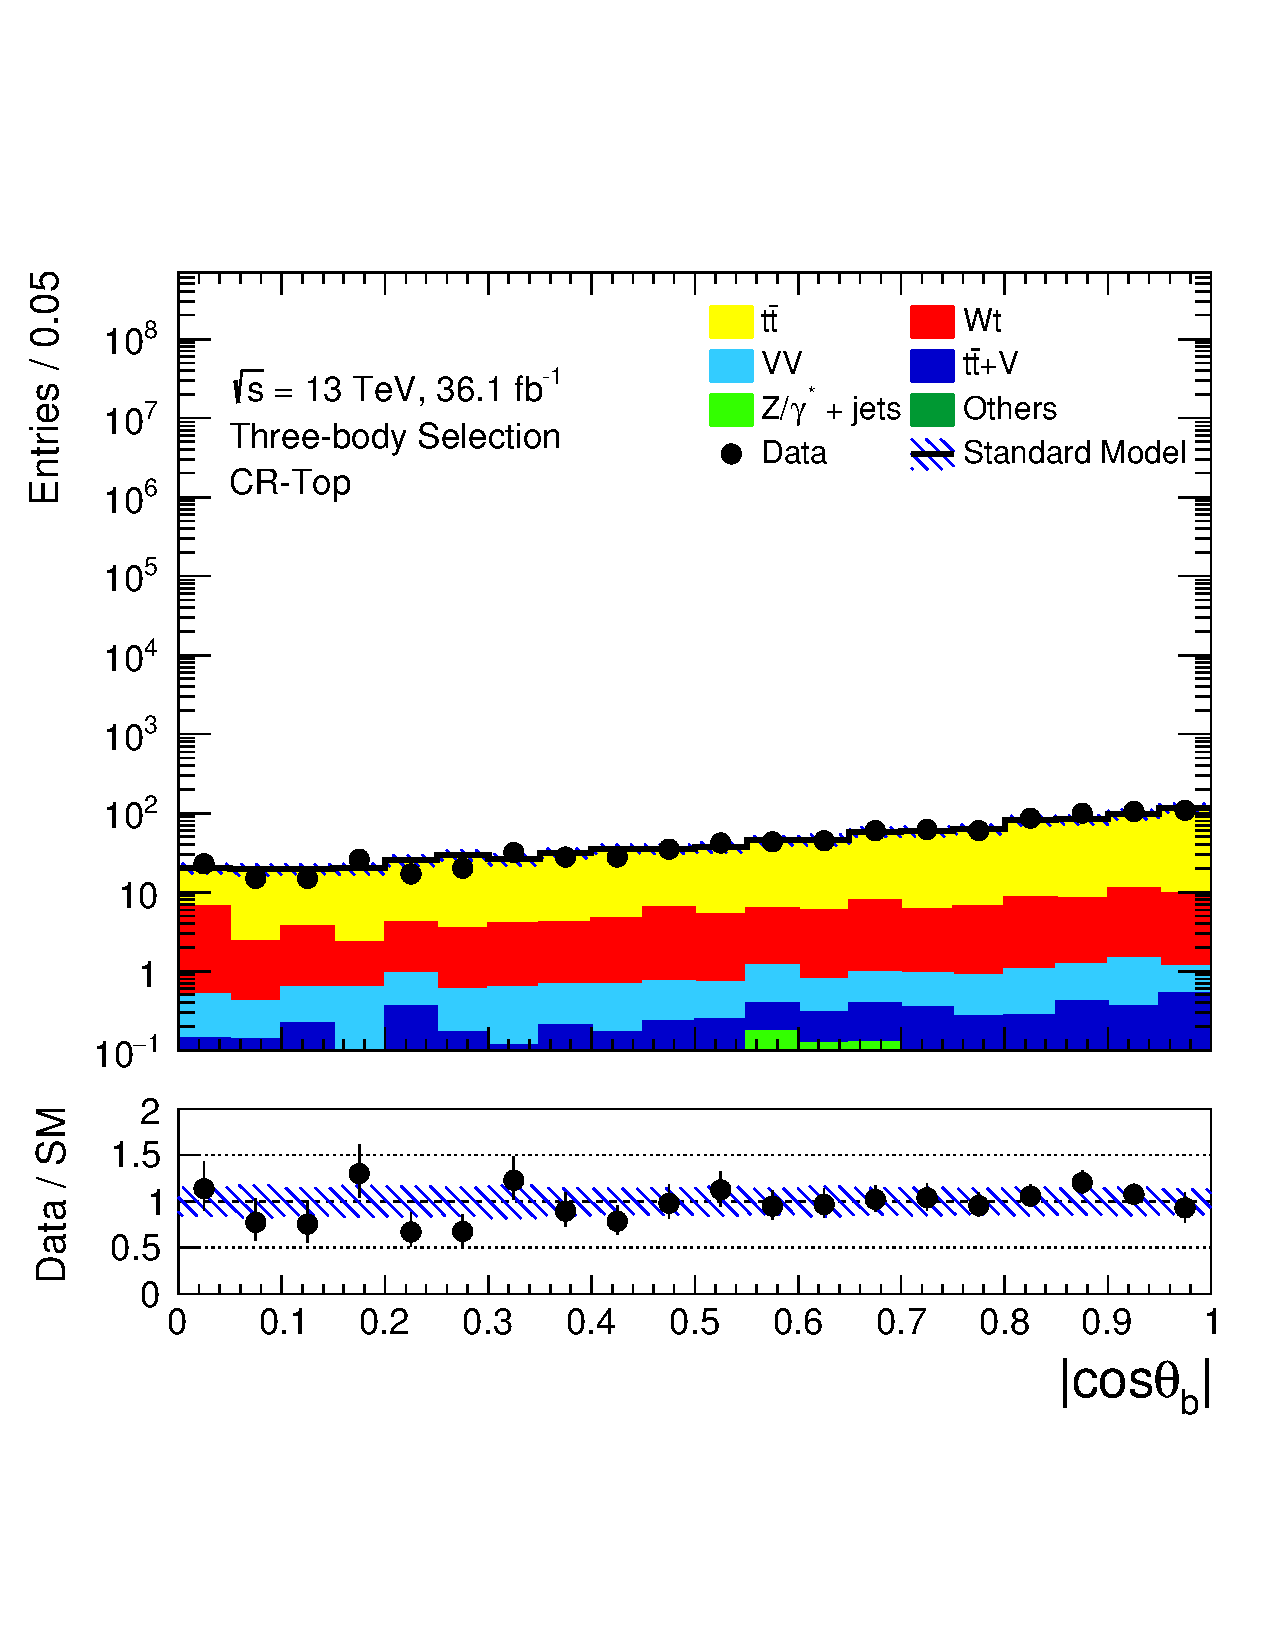
\includegraphics[width=0.48\textwidth]{figures/search_stop2l/bkg_est/crtop/crt_cosThetaB}
        \caption{
            Distributions of \mdr (\textit{\textbf{upper left}}), leading lepton \pT~(\textit{\textbf{upper right}}),
            \dpb (\textit{\textbf{lower left}}), and $|\cosb|$ (\textit{\textbf{lower right}}) in the \ttbar CR,
            CR-Top.
            The error on the SM processes includes statistical and systematic uncertainties.
            The post-fit normalization correction factors for the \ttbar and diboson processes
            have been applied.
        }
        \label{fig:crt_0}
    \end{center}
\end{figure}
\begin{figure}[!htb]
    \begin{center}
        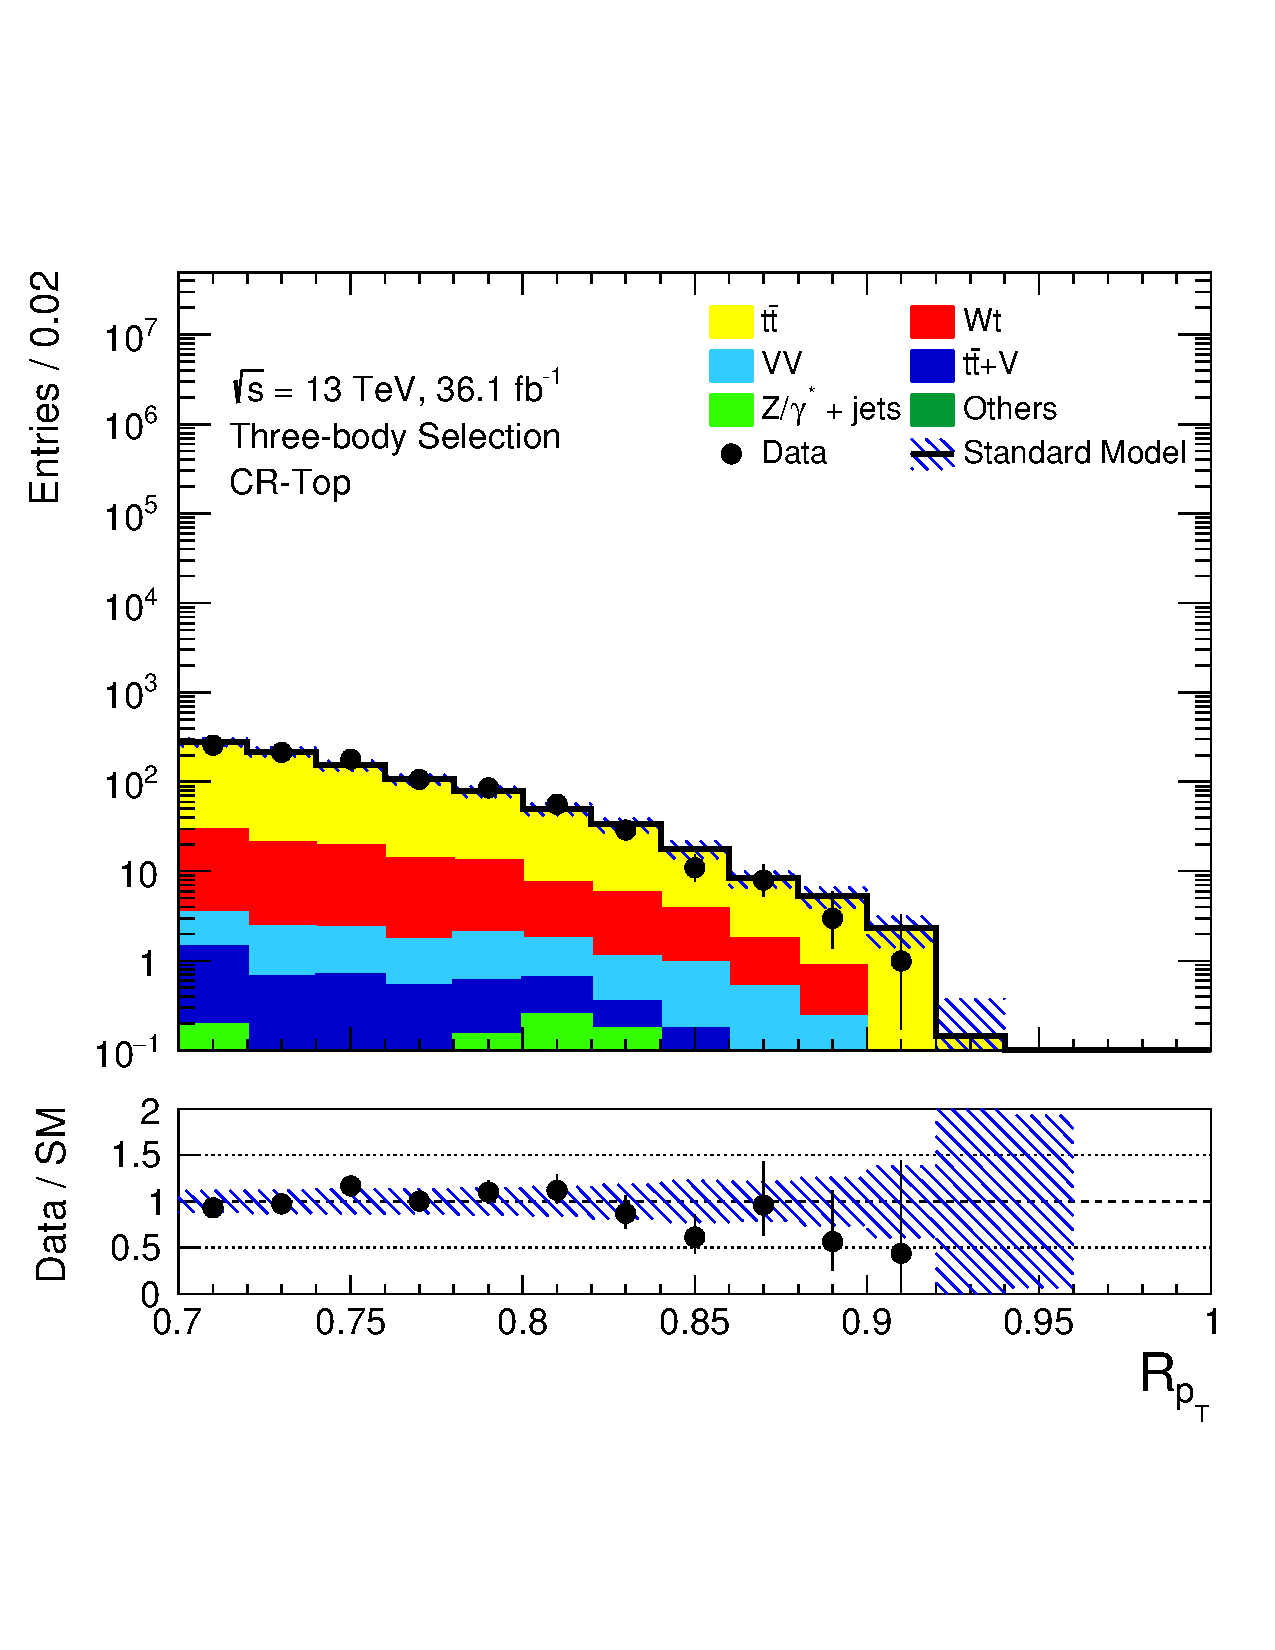
\includegraphics[width=0.48\textwidth]{figures/search_stop2l/bkg_est/crtop/crt_RPT}
        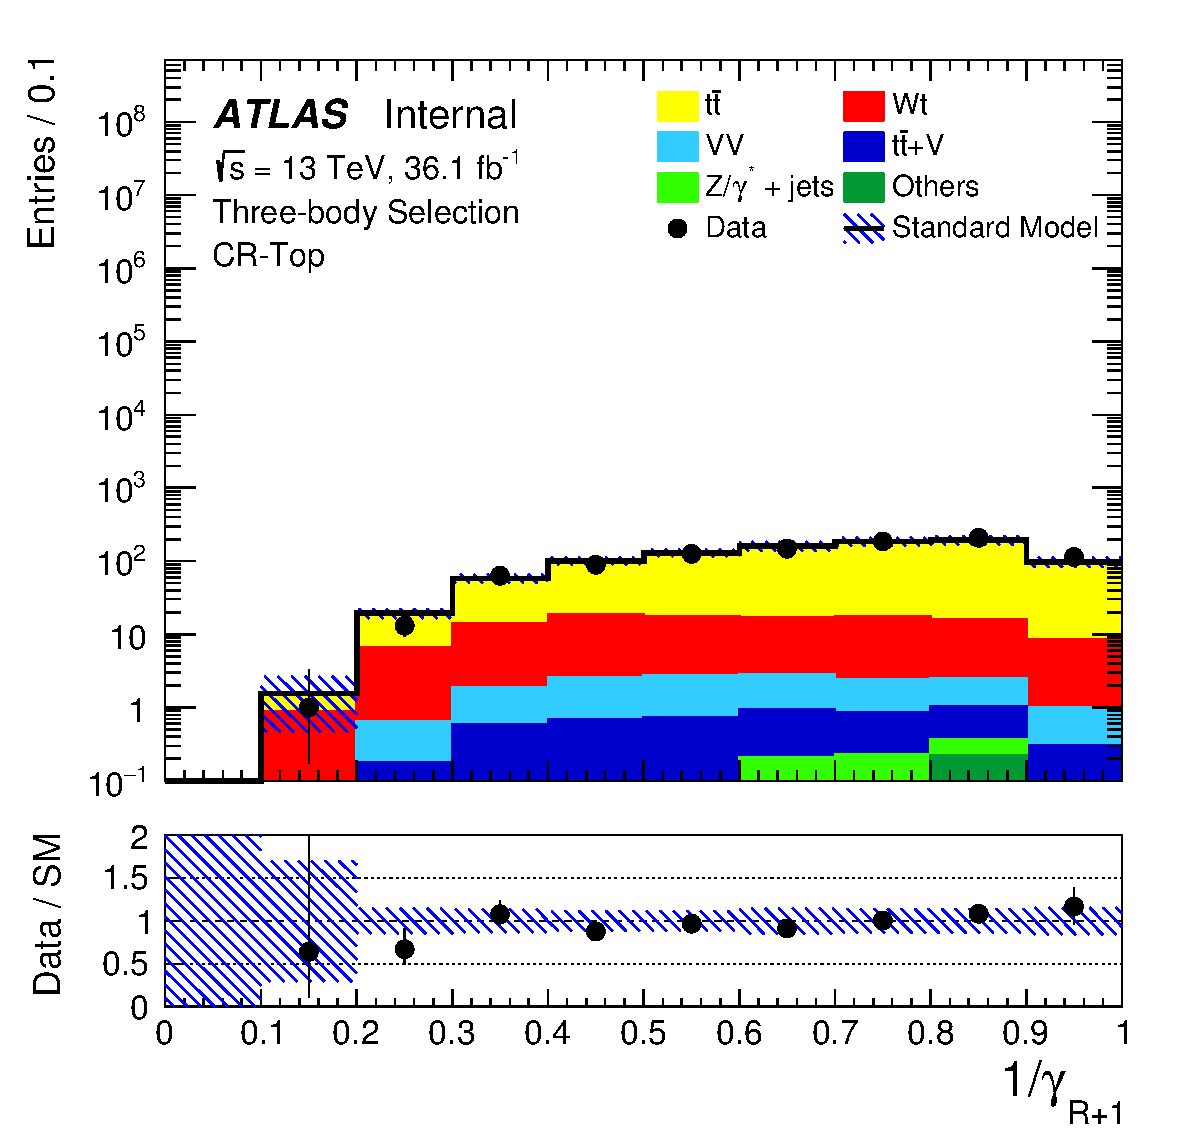
\includegraphics[width=0.48\textwidth]{figures/search_stop2l/bkg_est/crtop/crt_gamInvRp1}
        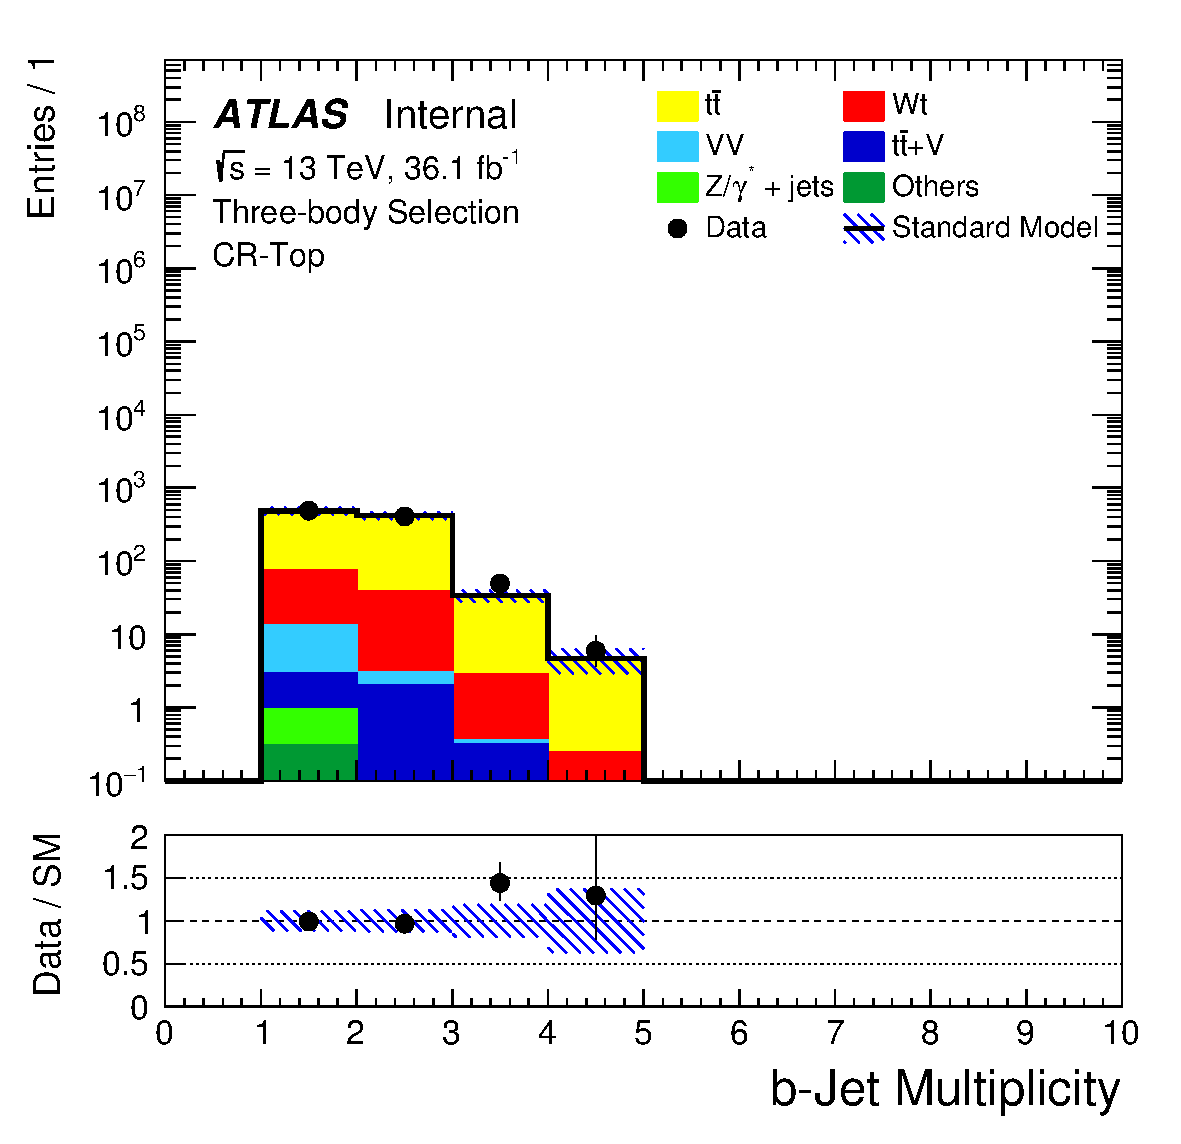
\includegraphics[width=0.48\textwidth]{figures/search_stop2l/bkg_est/crtop/crt_nBJets}
        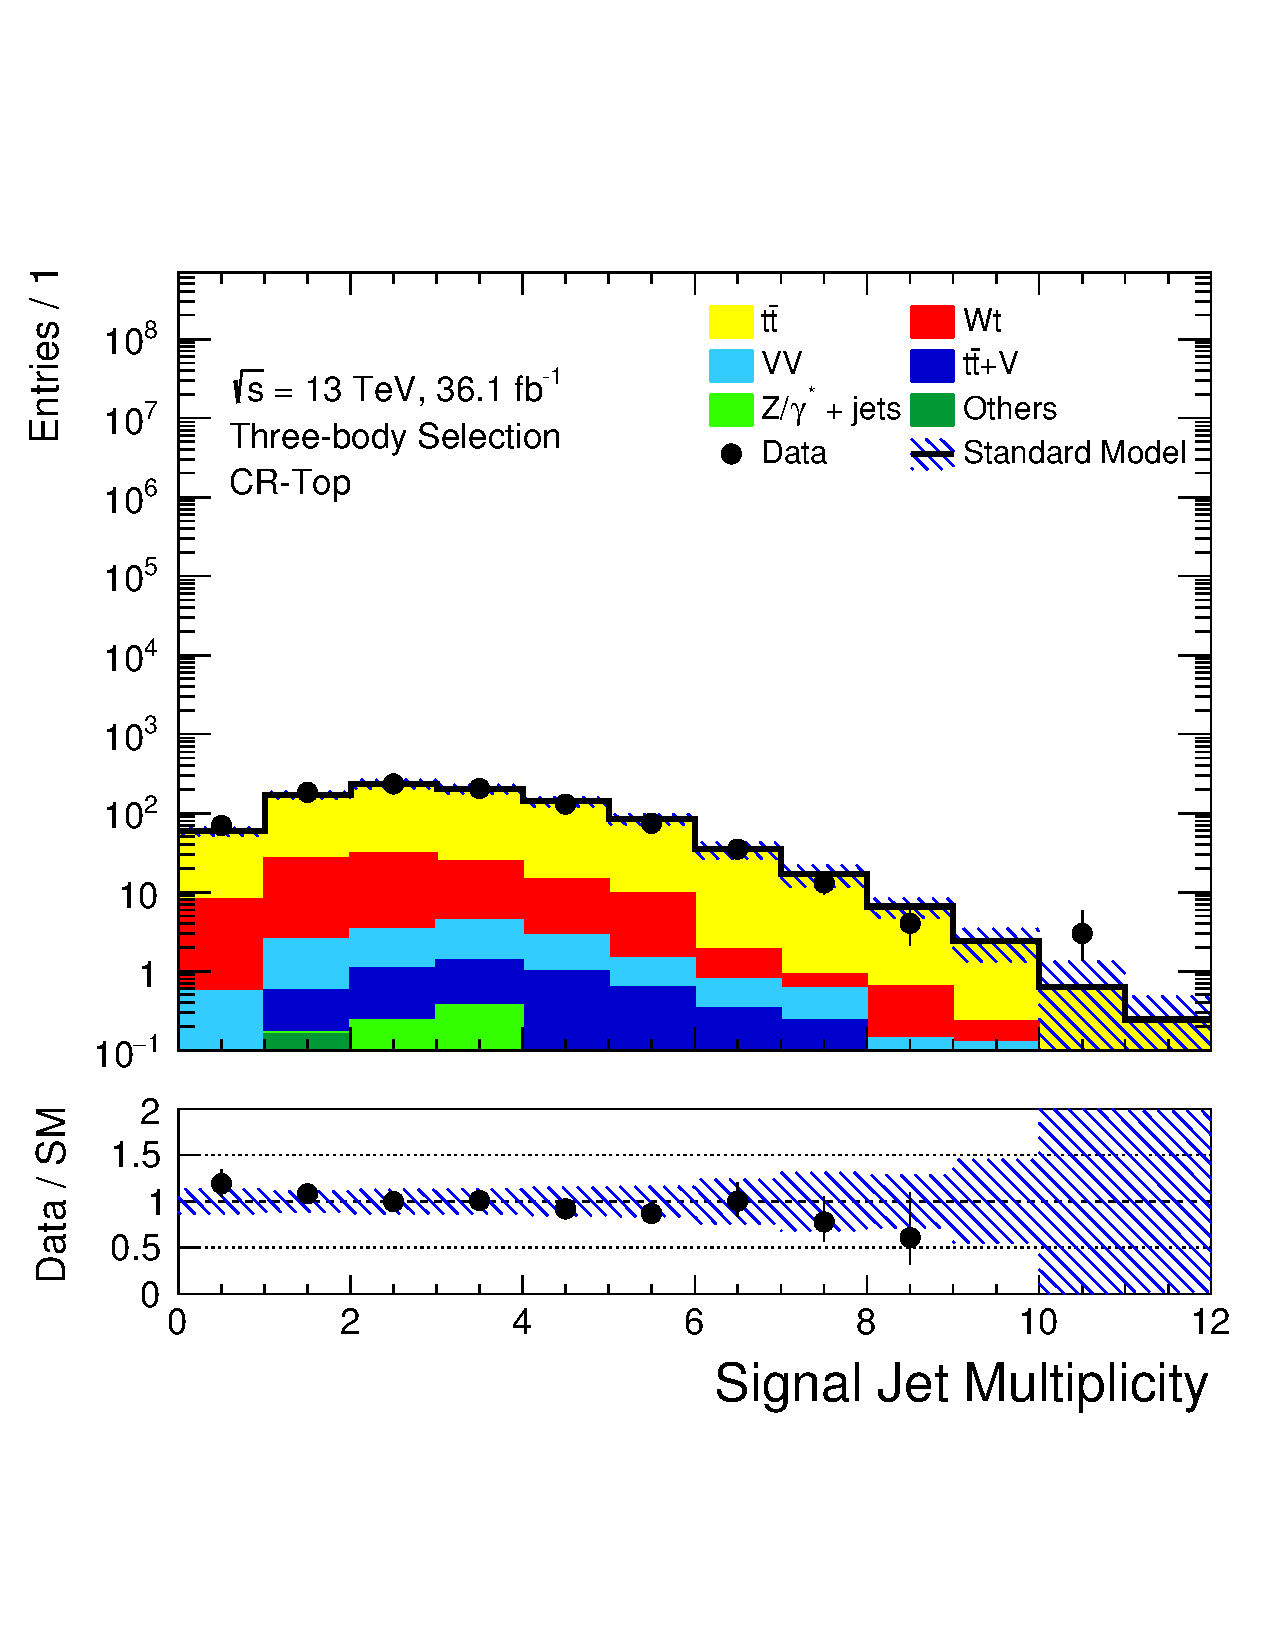
\includegraphics[width=0.48\textwidth]{figures/search_stop2l/bkg_est/crtop/crt_nSJets}
        \caption{
            Distributions of \rpt (\textit{\textbf{upper left}}), leading lepton \gaminv~(\textit{\textbf{upper right}}),
            $b$-tagged jet multiplicity (\textit{\textbf{lower left}}), and non-$b$-tagged jet multiplicity(\textit{\textbf{lower right}}) in the \ttbar CR,
            CR-Top.
            The error on the SM processes includes statistical and systematic uncertainties.
            The post-fit normalization correction factors for the \ttbar and diboson processes
            have been applied.
        }
        \label{fig:crt_1}
    \end{center}
\end{figure}



%%%%%%%%%%%%%%%%%%%%%%%%%%%%%%%%%%%%%%%%%%%%%%%%%%%%%%%%%%%%%%%%%%%%%%%%%%%%%%%%%%%%%%%%%%%%
%%%%%%%%%%%%%%%%%%%%%%%%%%%%%%%%%%%%%%%%%%%%%%%%%%%%%%%%%%%%%%%%%%%%%%%%%%%%%%%%%%%%%%%%%%%%
%%%%%%%%%%%%%%%%%%%%%%%%%%%%%%%%%%%%%%%%%%%%%%%%%%%%%%%%%%%%%%%%%%%%%%%%%%%%%%%%%%%%%%%%%%%%
%
% VV BKG
%
%%%%%%%%%%%%%%%%%%%%%%%%%%%%%%%%%%%%%%%%%%%%%%%%%%%%%%%%%%%%%%%%%%%%%%%%%%%%%%%%%%%%%%%%%%%%
%%%%%%%%%%%%%%%%%%%%%%%%%%%%%%%%%%%%%%%%%%%%%%%%%%%%%%%%%%%%%%%%%%%%%%%%%%%%%%%%%%%%%%%%%%%%
%%%%%%%%%%%%%%%%%%%%%%%%%%%%%%%%%%%%%%%%%%%%%%%%%%%%%%%%%%%%%%%%%%%%%%%%%%%%%%%%%%%%%%%%%%%%

\subsection{Diboson Production}
\label{sec:stop_vv_estimate}

The SM diboson processes are composed of $WW$, $ZW+WZ$, and $ZZ$ production.
The dominant process for the \bWN SRs is $WW$, as discussed in the text.
In order to constrain the $WW$ component, in addition to those components with a $Z$ boson,
the diboson CRs are split into two, one targeting the different-flavor enriched component
of the diboson background (predominantly $WW$) and one in which the same-flavor component ($ZW+WZ$ and $ZZ$)
is enriched.

The same-flavor and different-flavor diboson CRs (VRs), CR-VV-SF and CR-VV-DF (VR-VV-SF and VR-VV-DF), respectively,
are defined in Table~\ref{tab:stop_vv_crvr}.
All of the regions apply a $b$-tagged jet veto.
Although there are SRs that are inclusive of $b$-tagged jets (SRt-SF and SRt-DF), the diboson background
is negligible in them and so the normalisation correction factors derived in the diboson CRs
can be extrapolated with confidence into the SRs with a $b$-tagged jet veto (SRw-SF and SRw-DF).
There is no difference between the same-flavor and different-flavor CRs, apart from the dilepton flavor
requirements and $Z$-veto.
The diboson VRs have the same, or inclusive, \rpt and \gaminv  selections as the CRs but have orthogonal
\mdr requirements that move them closer the SR selections.

Distributions of several key observables in CR-VV-SF (CR-VV-DF) are shown in Figures~\ref{fig:crvvSF_0}-\ref{fig:crvvSF_1}
(Figures~\ref{fig:crvvDF_0}-\ref{fig:crvvDF_1}).

\begin{table}[!htb]
    \begin{center}
        \begin{scriptsize}
        \caption{
            Definitions of the CR and VR for the diboson~background processes for the
            \bWN search.
        }
        \label{tab:stop_vv_crvr}
        \begin{tabular}{l | c c c c}
            \hline
            \hline
                & \multicolumn{4}{c}{\textbf{Regions}} \\
            \hline
            \textbf{Variable} & \textbf{CR-VV-DF} & \textbf{CR-VV-SF} & \textbf{VR-VV-DF} & \textbf{VR-VV-SF} \\
            \hline
            Dilepton Flavor & DF & SF & DF & SF \\
            $m_{\ell\ell}$ [GeV]    & no req. & $|m_{\ell\ell} - 91.2| > 10$ & no req. & $|m_{\ell\ell} - 91.2| > 10$ \\
            Lead lepton \pT~[GeV] & $>25$ & $>25$ & $>25$ & $>25$ \\
            Sub-lead lepton \pT~[GeV] & $>20$ & $>20$ & $>20$ & $>20$ \\
            $b$-tagged jet multiplicity & Exactly 0 & Exactly 0 & Exactly 0 & Exactly 0 \\
            \mdr [GeV] & $>50$ & $>70$ & $\in(50,95)$ & $\in(60,95)$ \\
            \rpt & $<0.5$ & $<0.5$ & $<0.7$ & $<0.4$ \\
            \gaminv &  $>0.7$ & $>0.7$ & $>0.7$ & $>0.7$ \\
            $(\cosb, \dpb)$ & \multicolumn{2}{c}{\small{$\dpb < 0.9 \times | \cosb | + 1.6$}} & \multicolumn{2}{c}{\small{$\dpb> 0.9 \times | \cosb | + 1.6$}} \\
            \hline
            \hline
        \end{tabular}
        \end{scriptsize}
    \end{center}
\end{table}

\begin{figure}[!htb]
    \begin{center}
        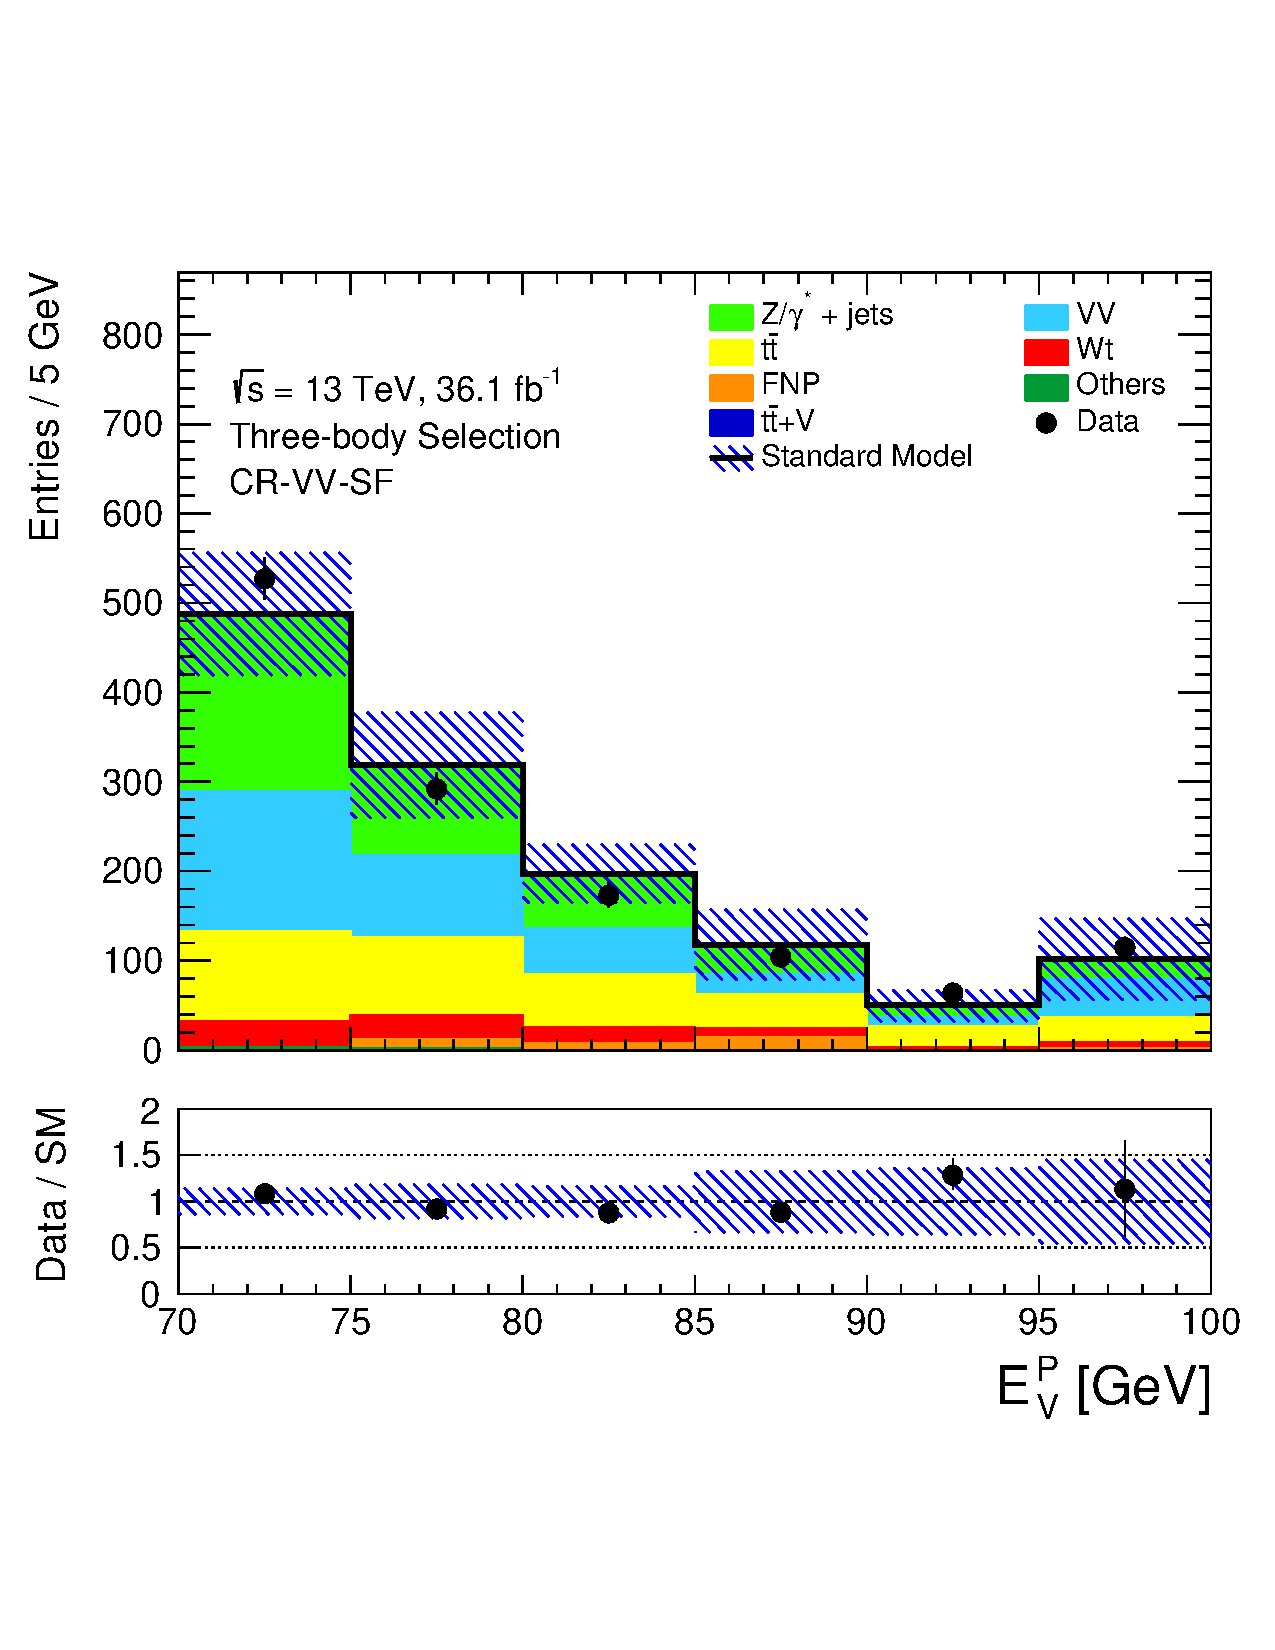
\includegraphics[width=0.48\textwidth]{figures/search_stop2l/bkg_est/crvsf/crvSF_MDR}
        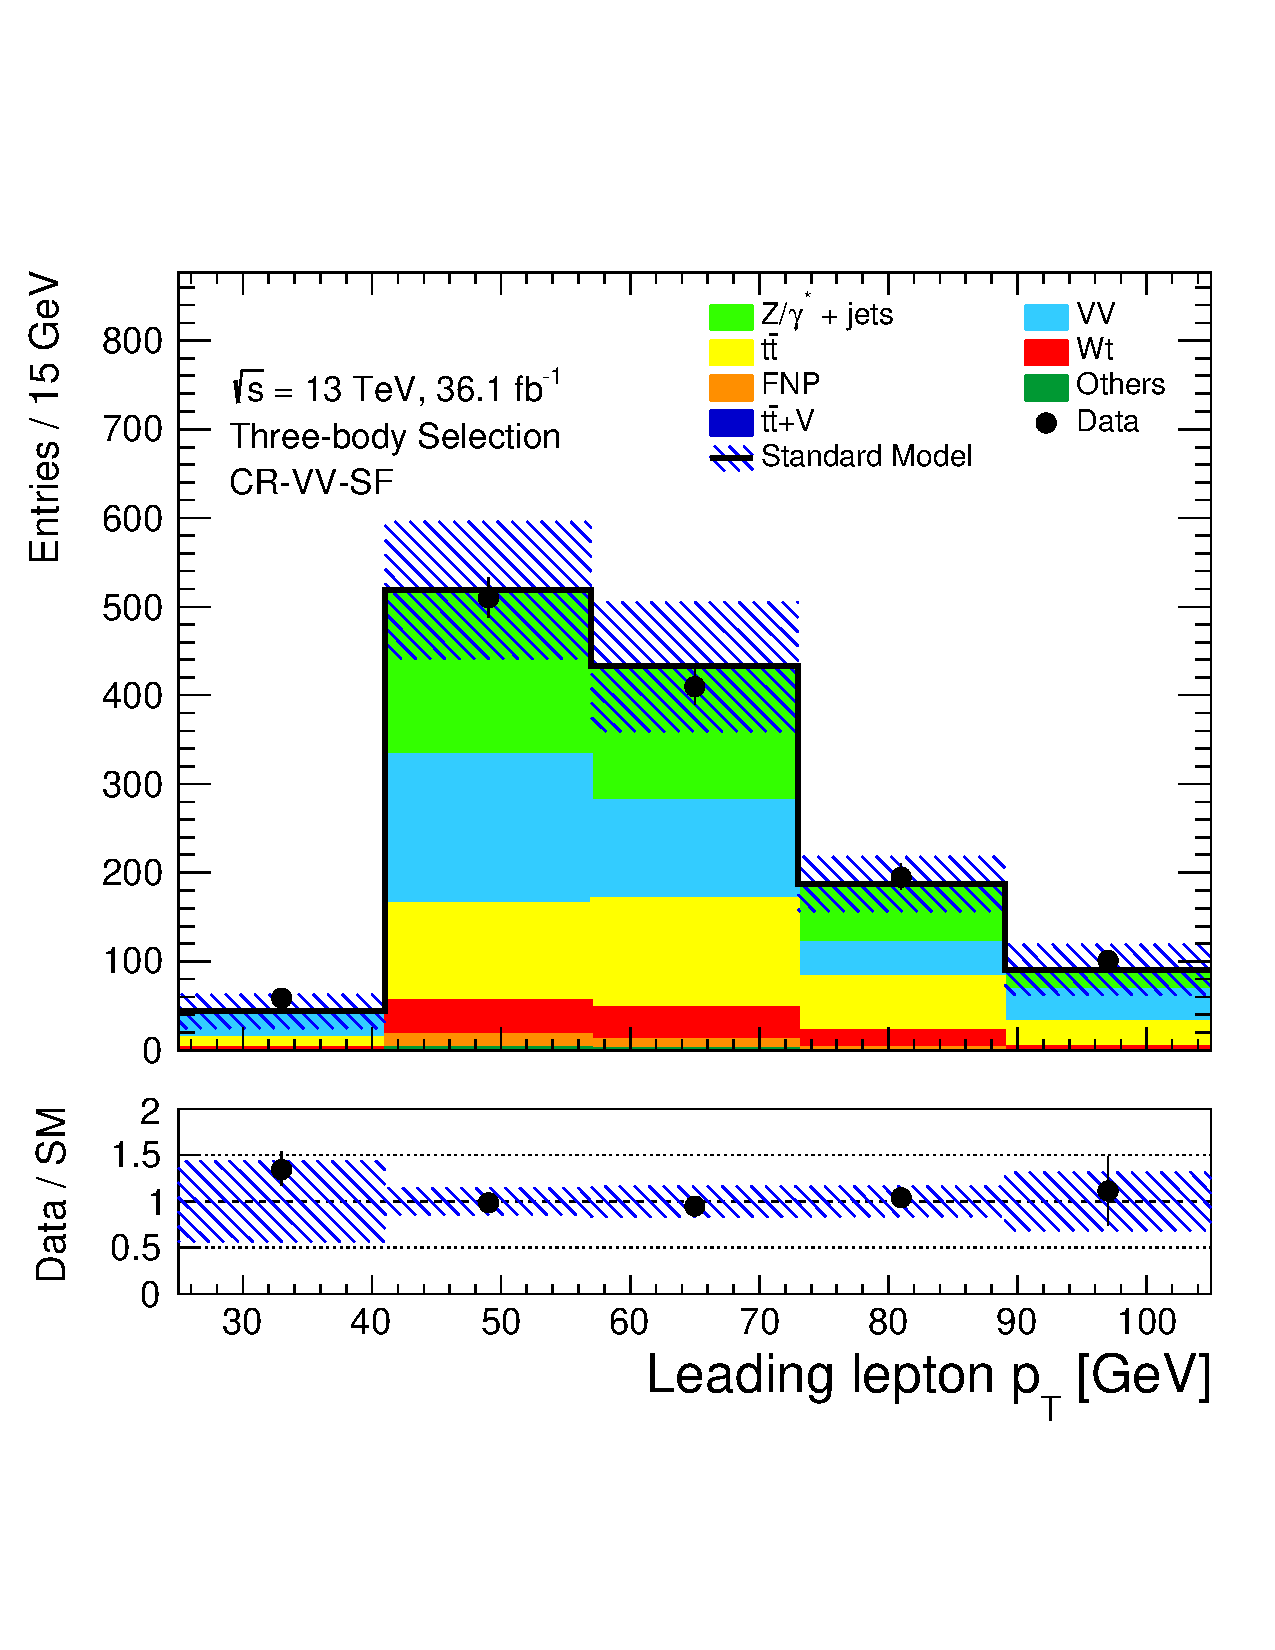
\includegraphics[width=0.48\textwidth]{figures/search_stop2l/bkg_est/crvsf/crvSF_l_pt0}
        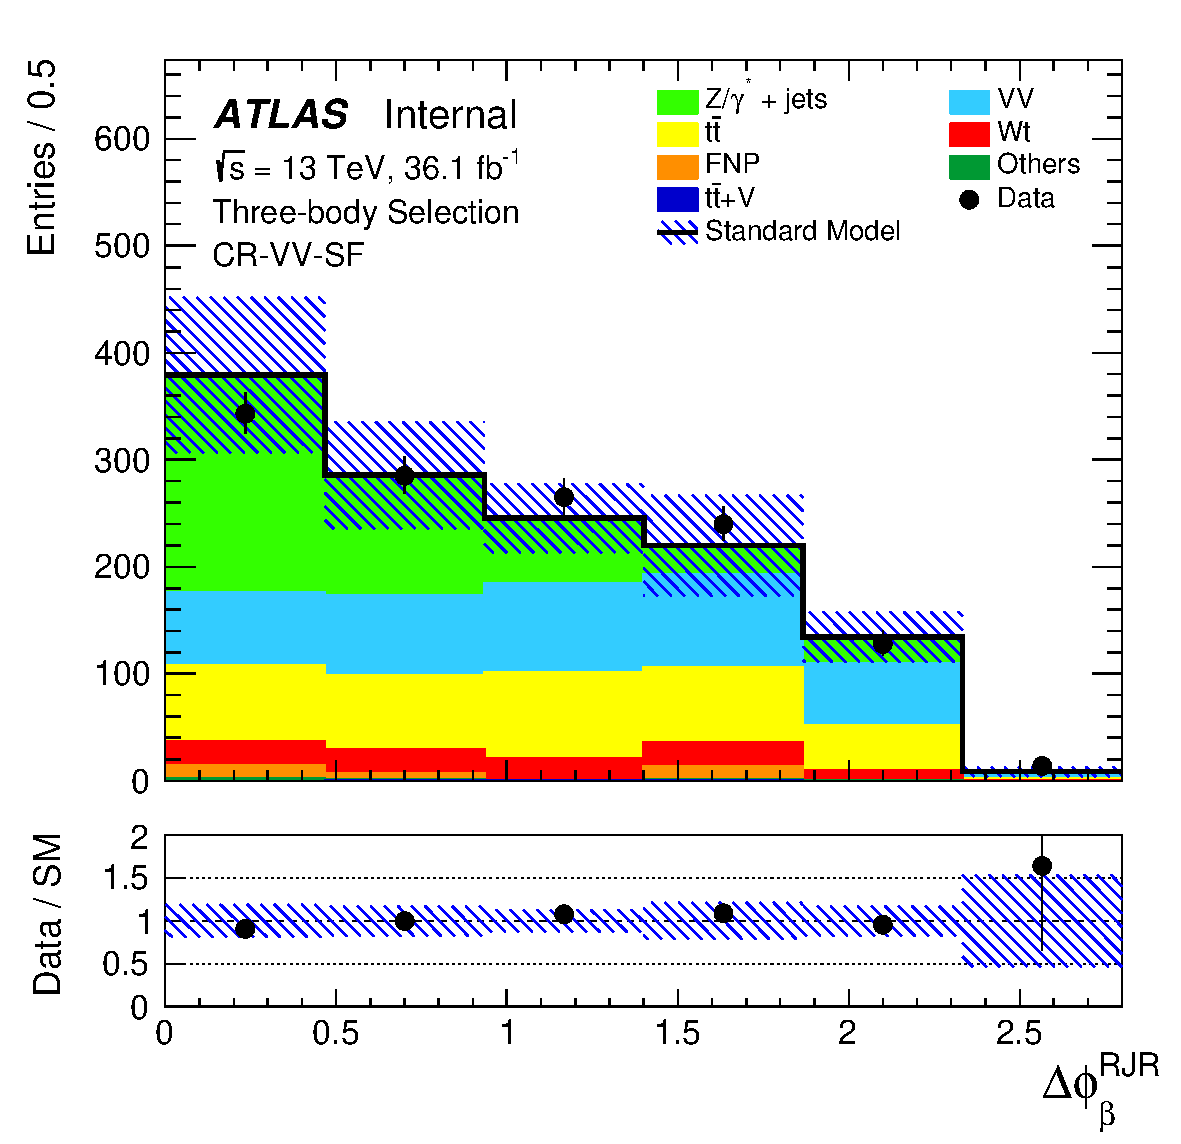
\includegraphics[width=0.48\textwidth]{figures/search_stop2l/bkg_est/crvsf/crvSF_DPB_vSS}
        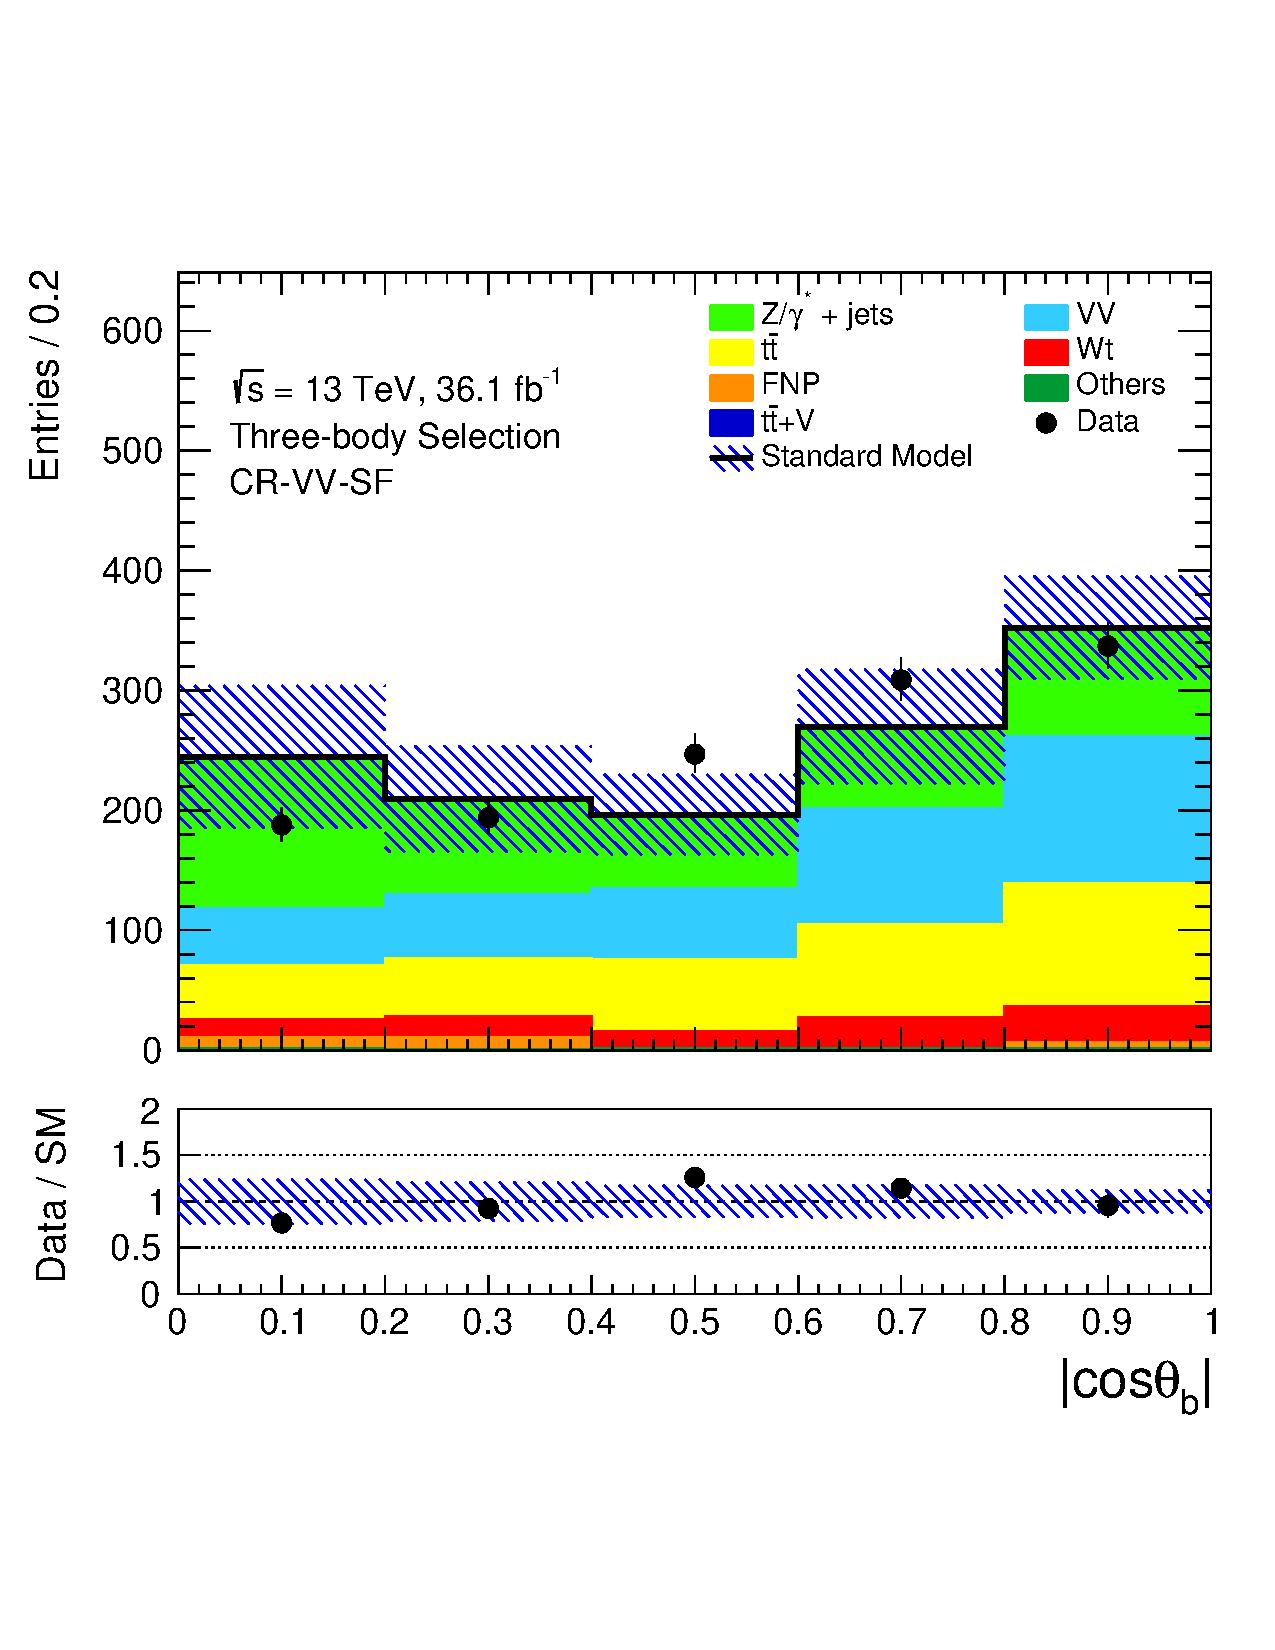
\includegraphics[width=0.48\textwidth]{figures/search_stop2l/bkg_est/crvsf/crvSF_cosThetaB}
        \caption{
            Distributions of \mdr (\textit{\textbf{upper left}}), leading lepton \pT~(\textit{\textbf{upper right}}),
            \dpb (\textit{\textbf{lower left}}), and $|\cosb|$ (\textit{\textbf{lower right}}) in the same-flavor diboson CR,
            CR-VV-SF.
            The error on the SM processes includes statistical and systematic uncertainties.
            The post-fit normalization correction factors for the \ttbar and diboson processes
            have been applied.
        }
        \label{fig:crvvSF_0}
    \end{center}
\end{figure}
\begin{figure}[!htb]
    \begin{center}
        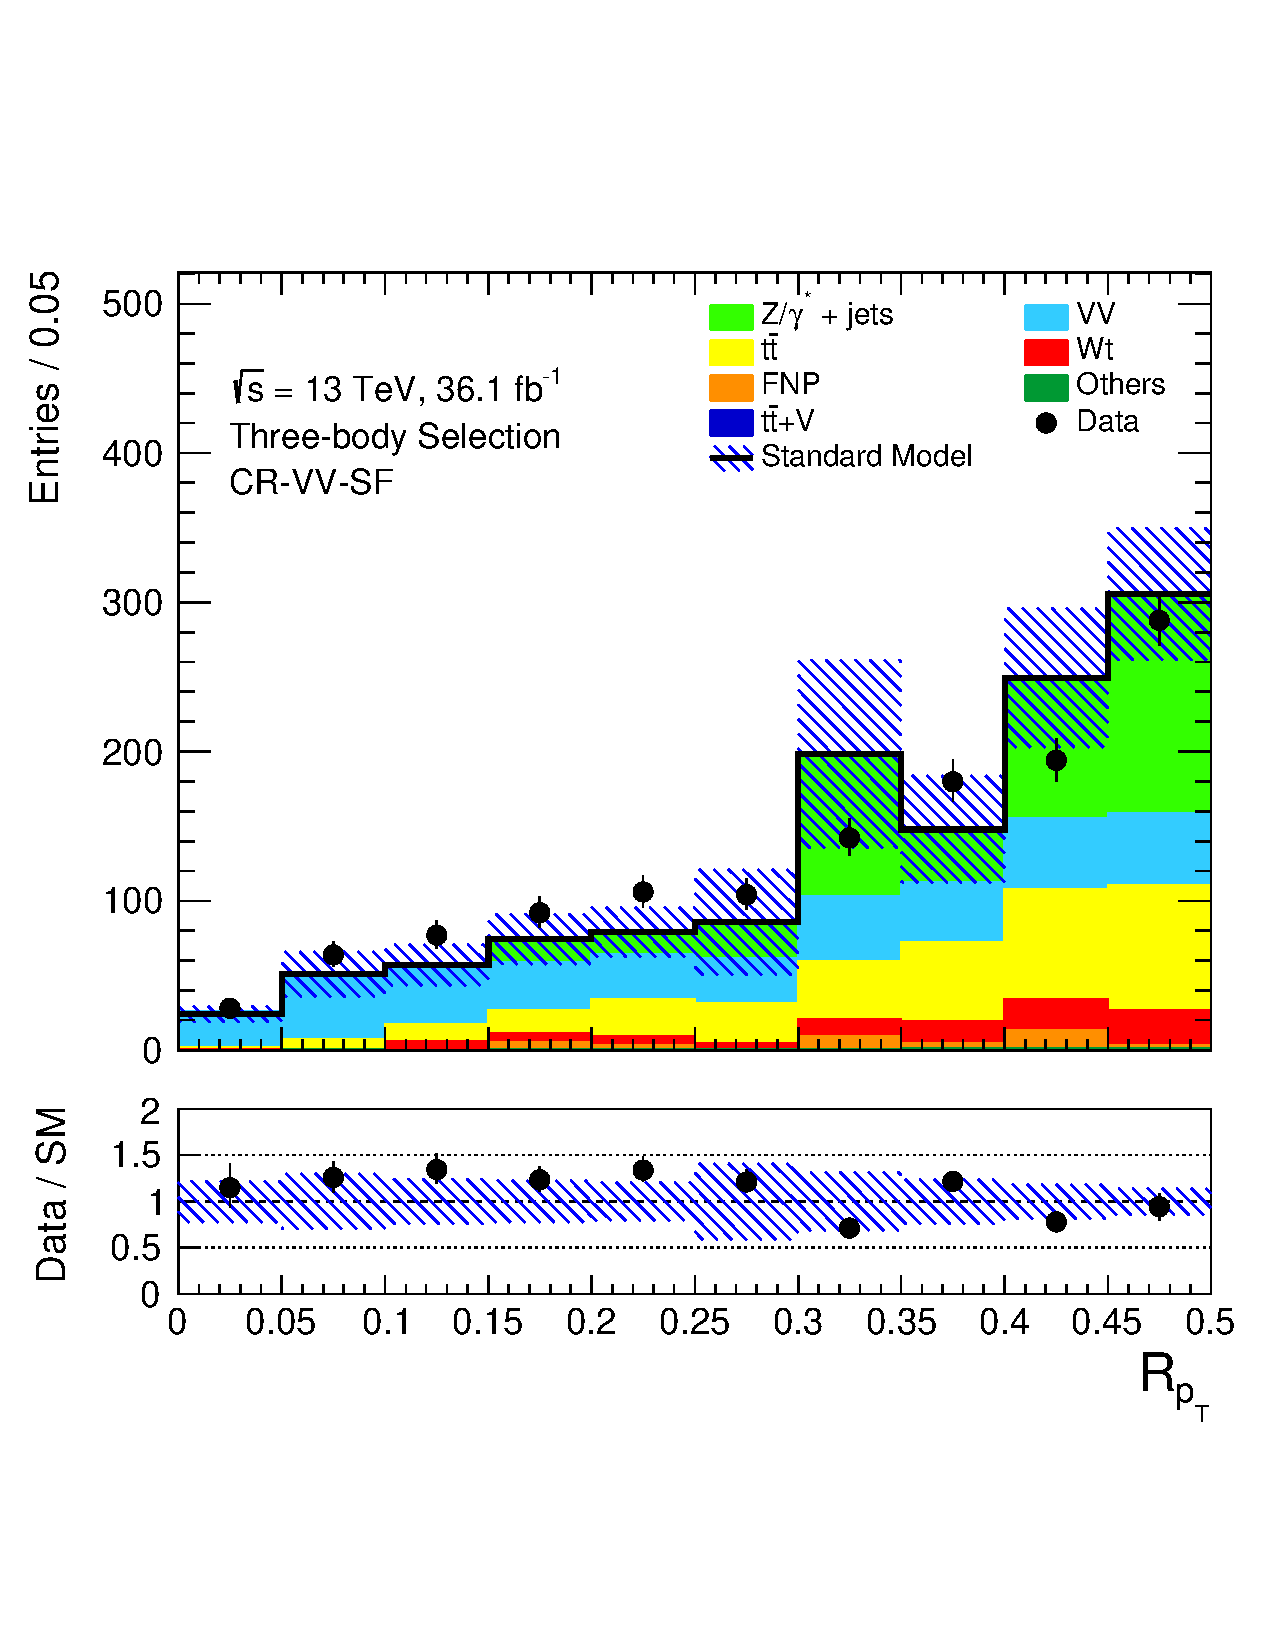
\includegraphics[width=0.48\textwidth]{figures/search_stop2l/bkg_est/crvsf/crvSF_RPT}
        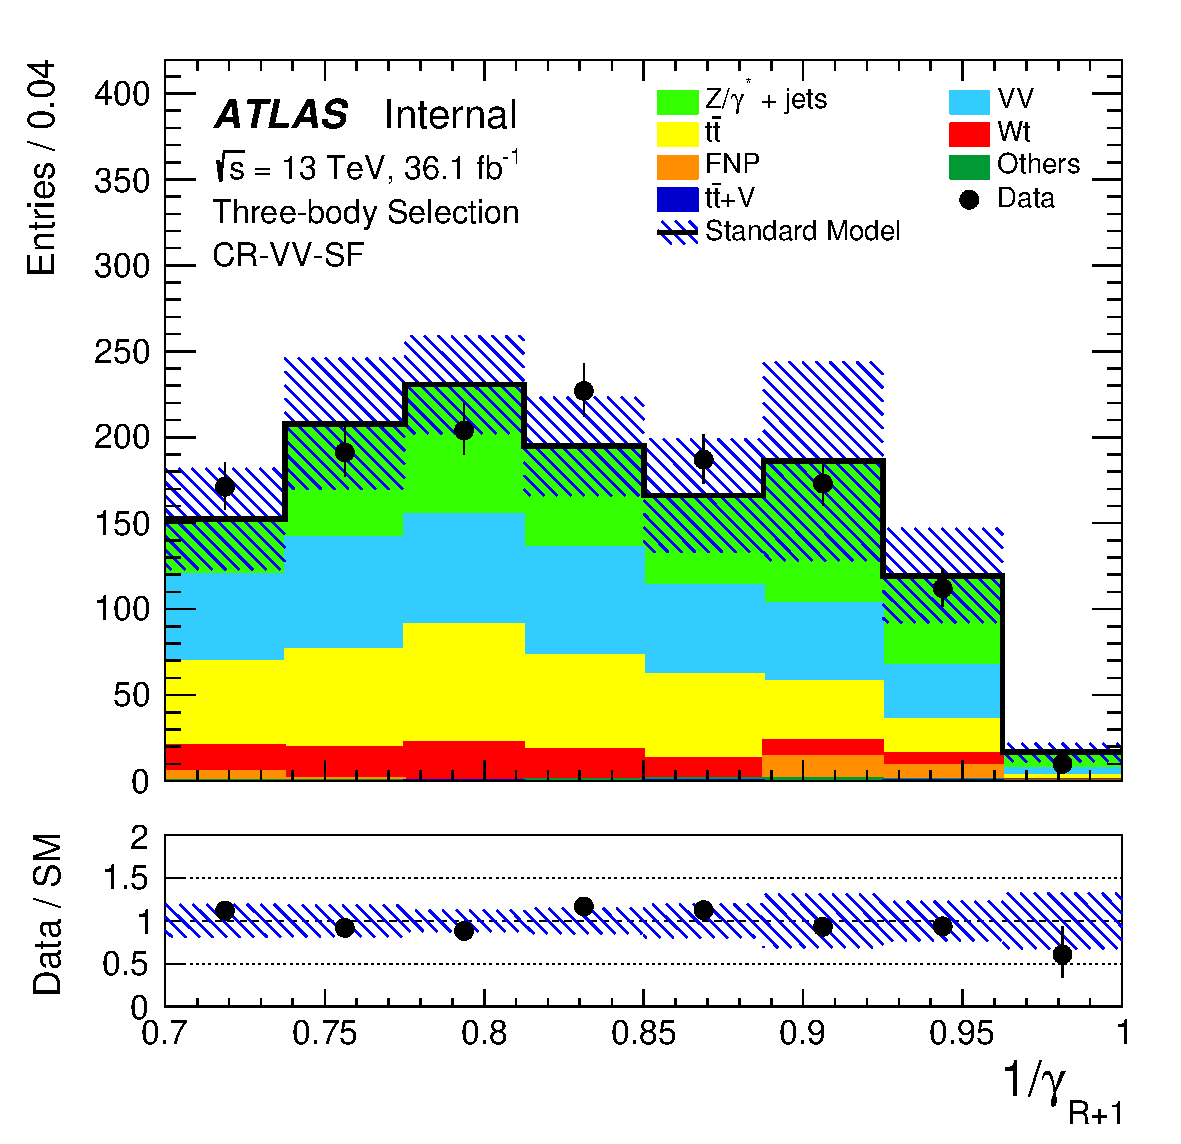
\includegraphics[width=0.48\textwidth]{figures/search_stop2l/bkg_est/crvsf/crvSF_gamInvRp1}
        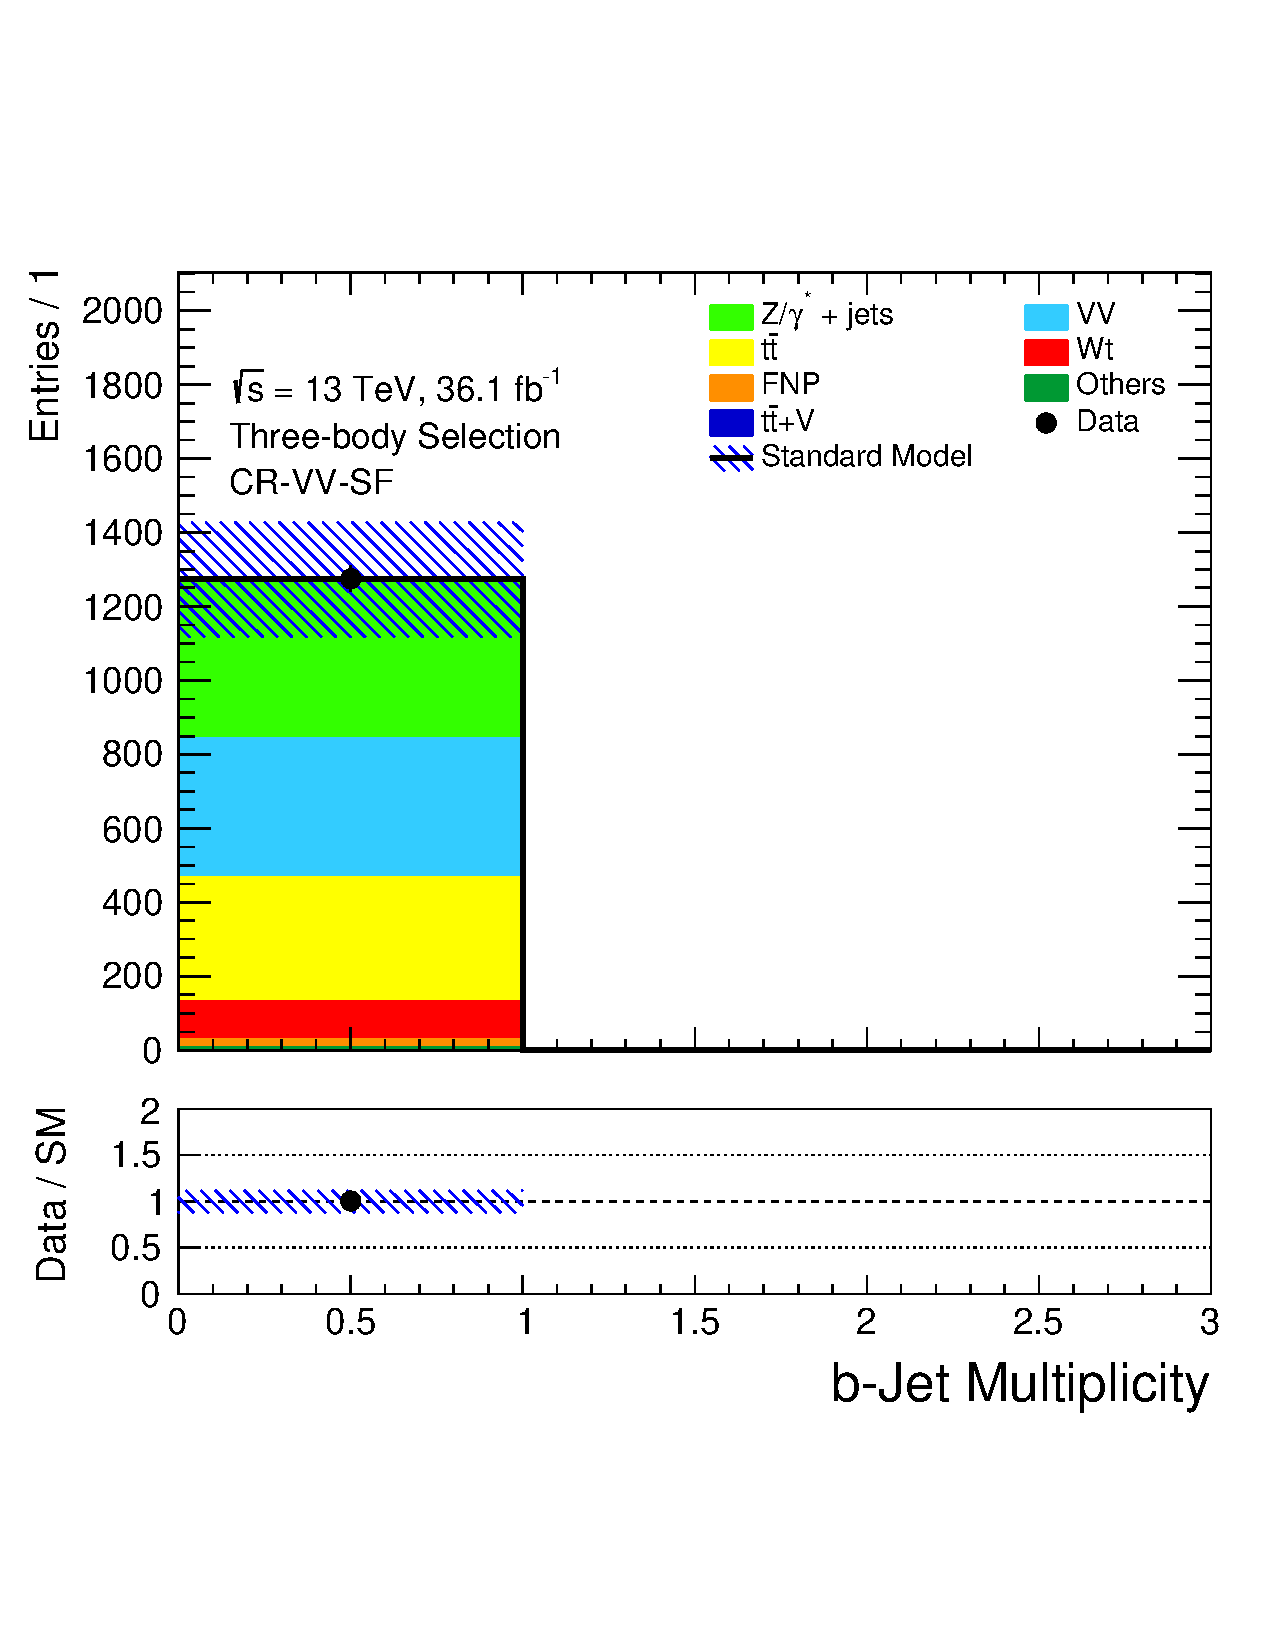
\includegraphics[width=0.48\textwidth]{figures/search_stop2l/bkg_est/crvsf/crvSF_nBJets}
        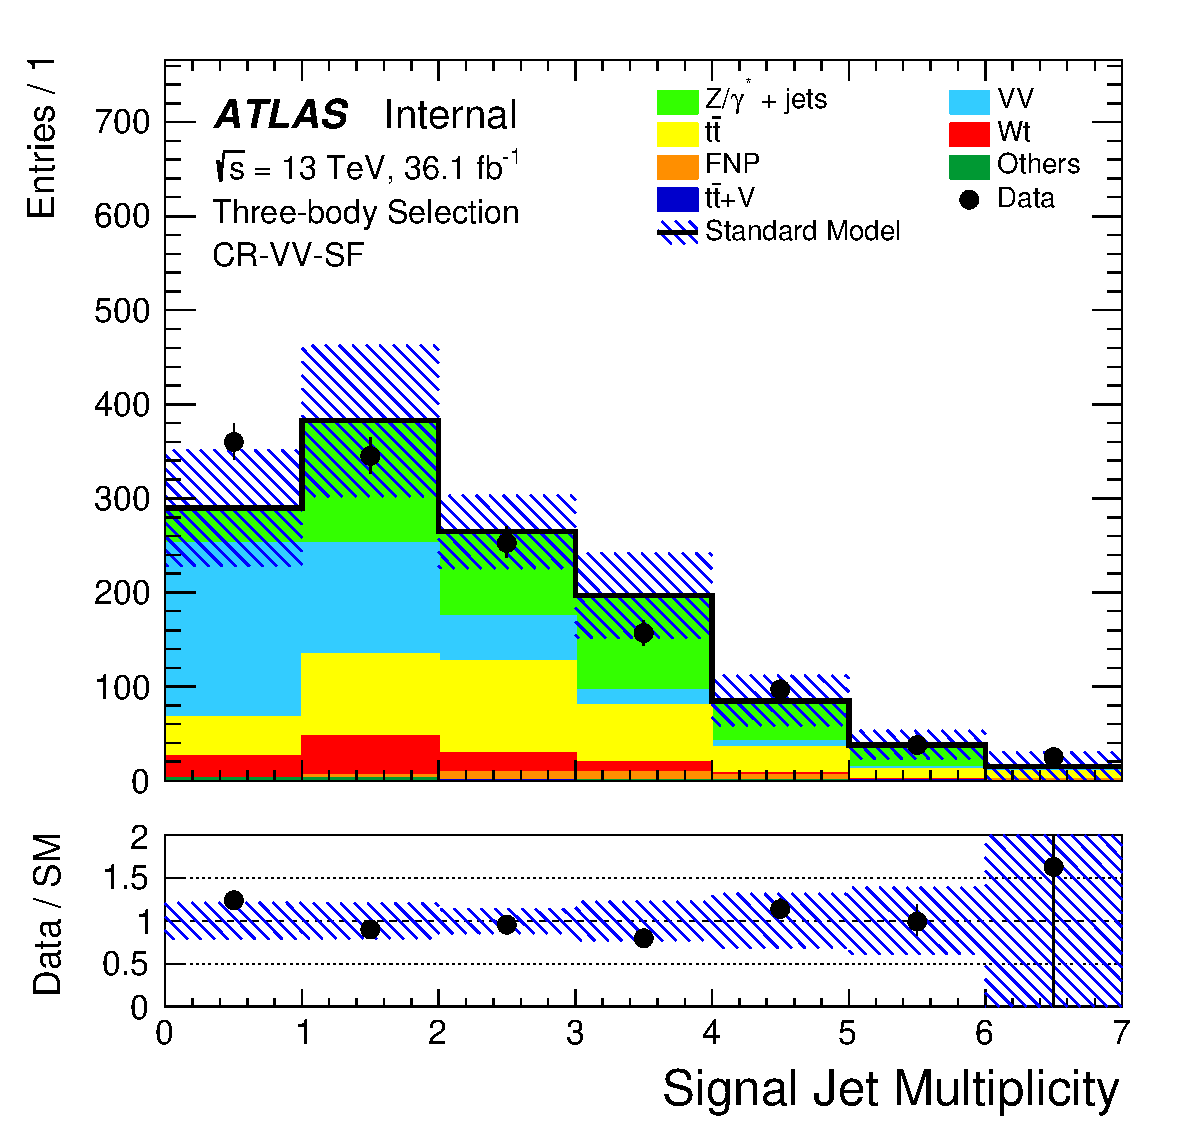
\includegraphics[width=0.48\textwidth]{figures/search_stop2l/bkg_est/crvsf/crvSF_nSJets}
        \caption{
            Distributions of \rpt (\textit{\textbf{upper left}}), leading lepton \gaminv~(\textit{\textbf{upper right}}),
            $b$-tagged jet multiplicity (\textit{\textbf{lower left}}), and non-$b$-tagged jet multiplicity(\textit{\textbf{lower right}}) in the same-flavor diboson CR,
            CR-VV-SF.
            The error on the SM processes includes statistical and systematic uncertainties.
            The post-fit normalization correction factors for the \ttbar and diboson processes
            have been applied.
        }
        \label{fig:crvvSF_1}
    \end{center}
\end{figure}

\begin{figure}[!htb]
    \begin{center}
        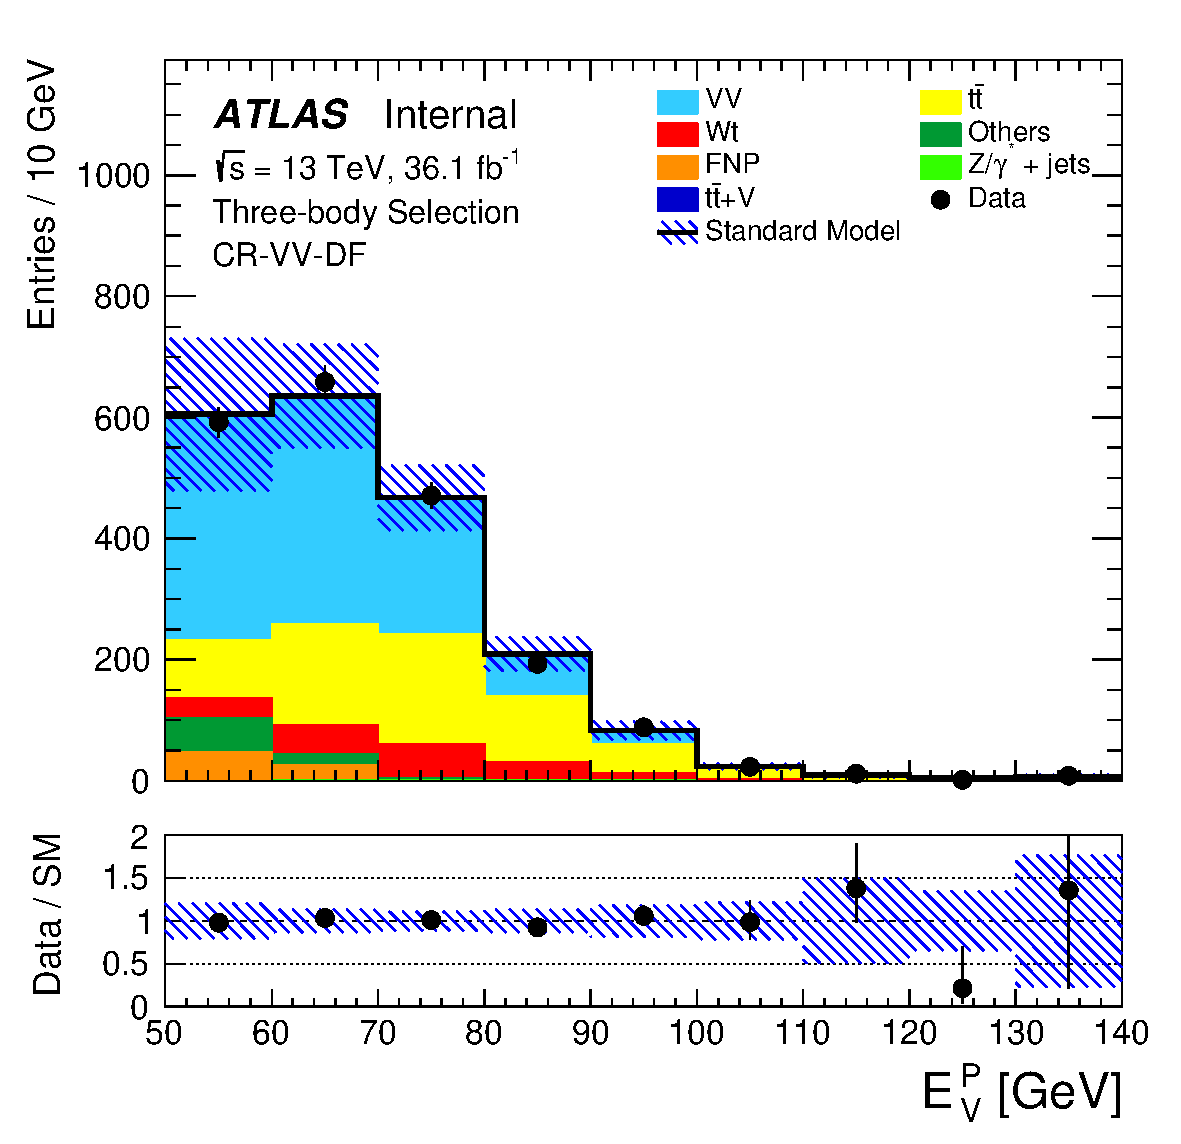
\includegraphics[width=0.48\textwidth]{figures/search_stop2l/bkg_est/crvdf/crv_MDR}
        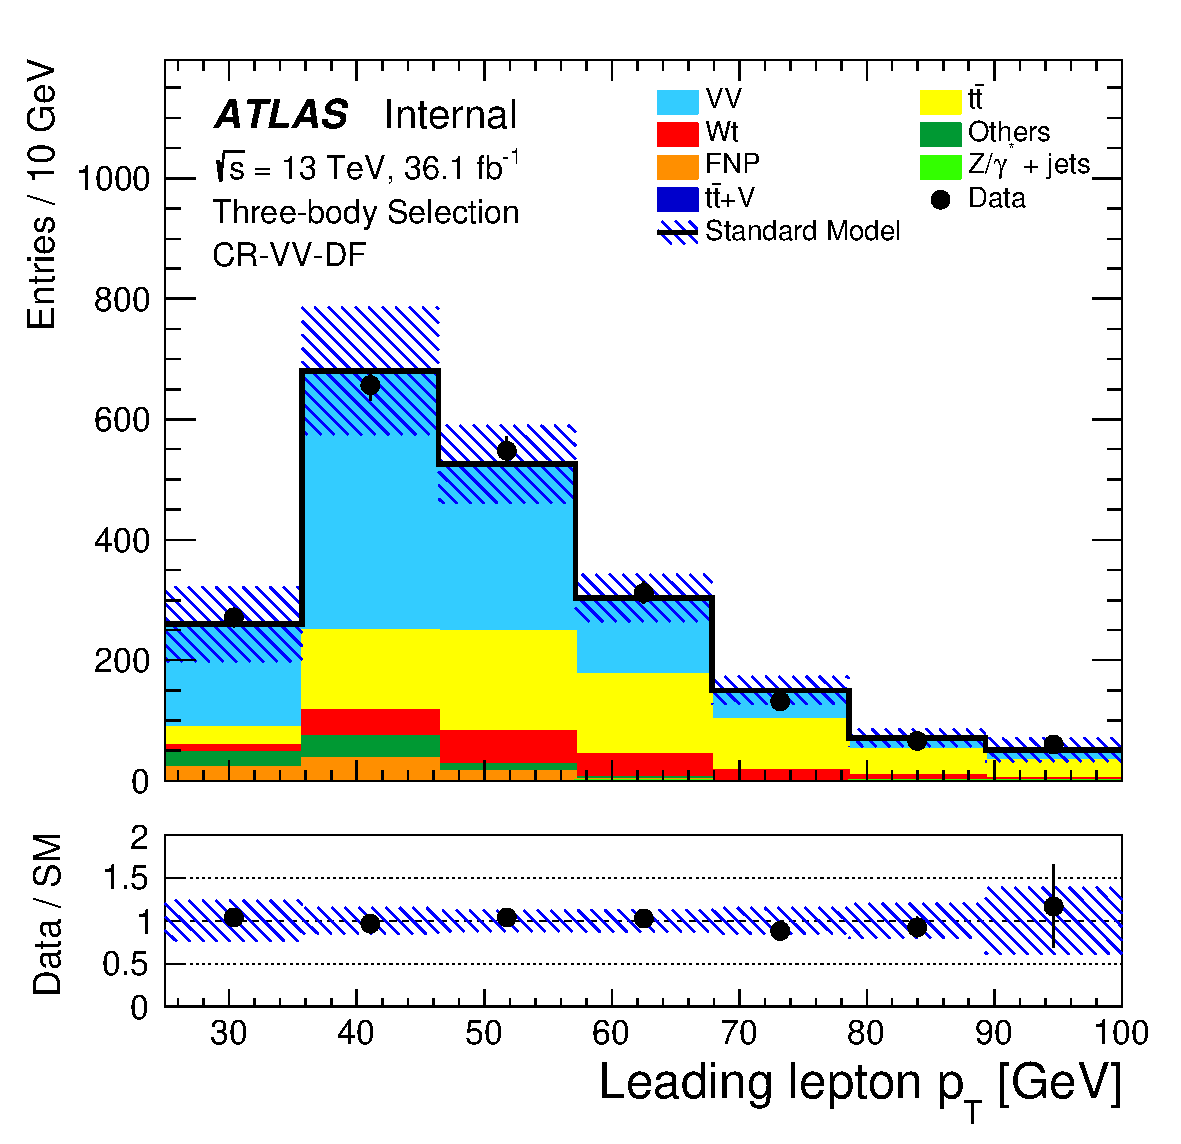
\includegraphics[width=0.48\textwidth]{figures/search_stop2l/bkg_est/crvdf/crv_l_pt0}
        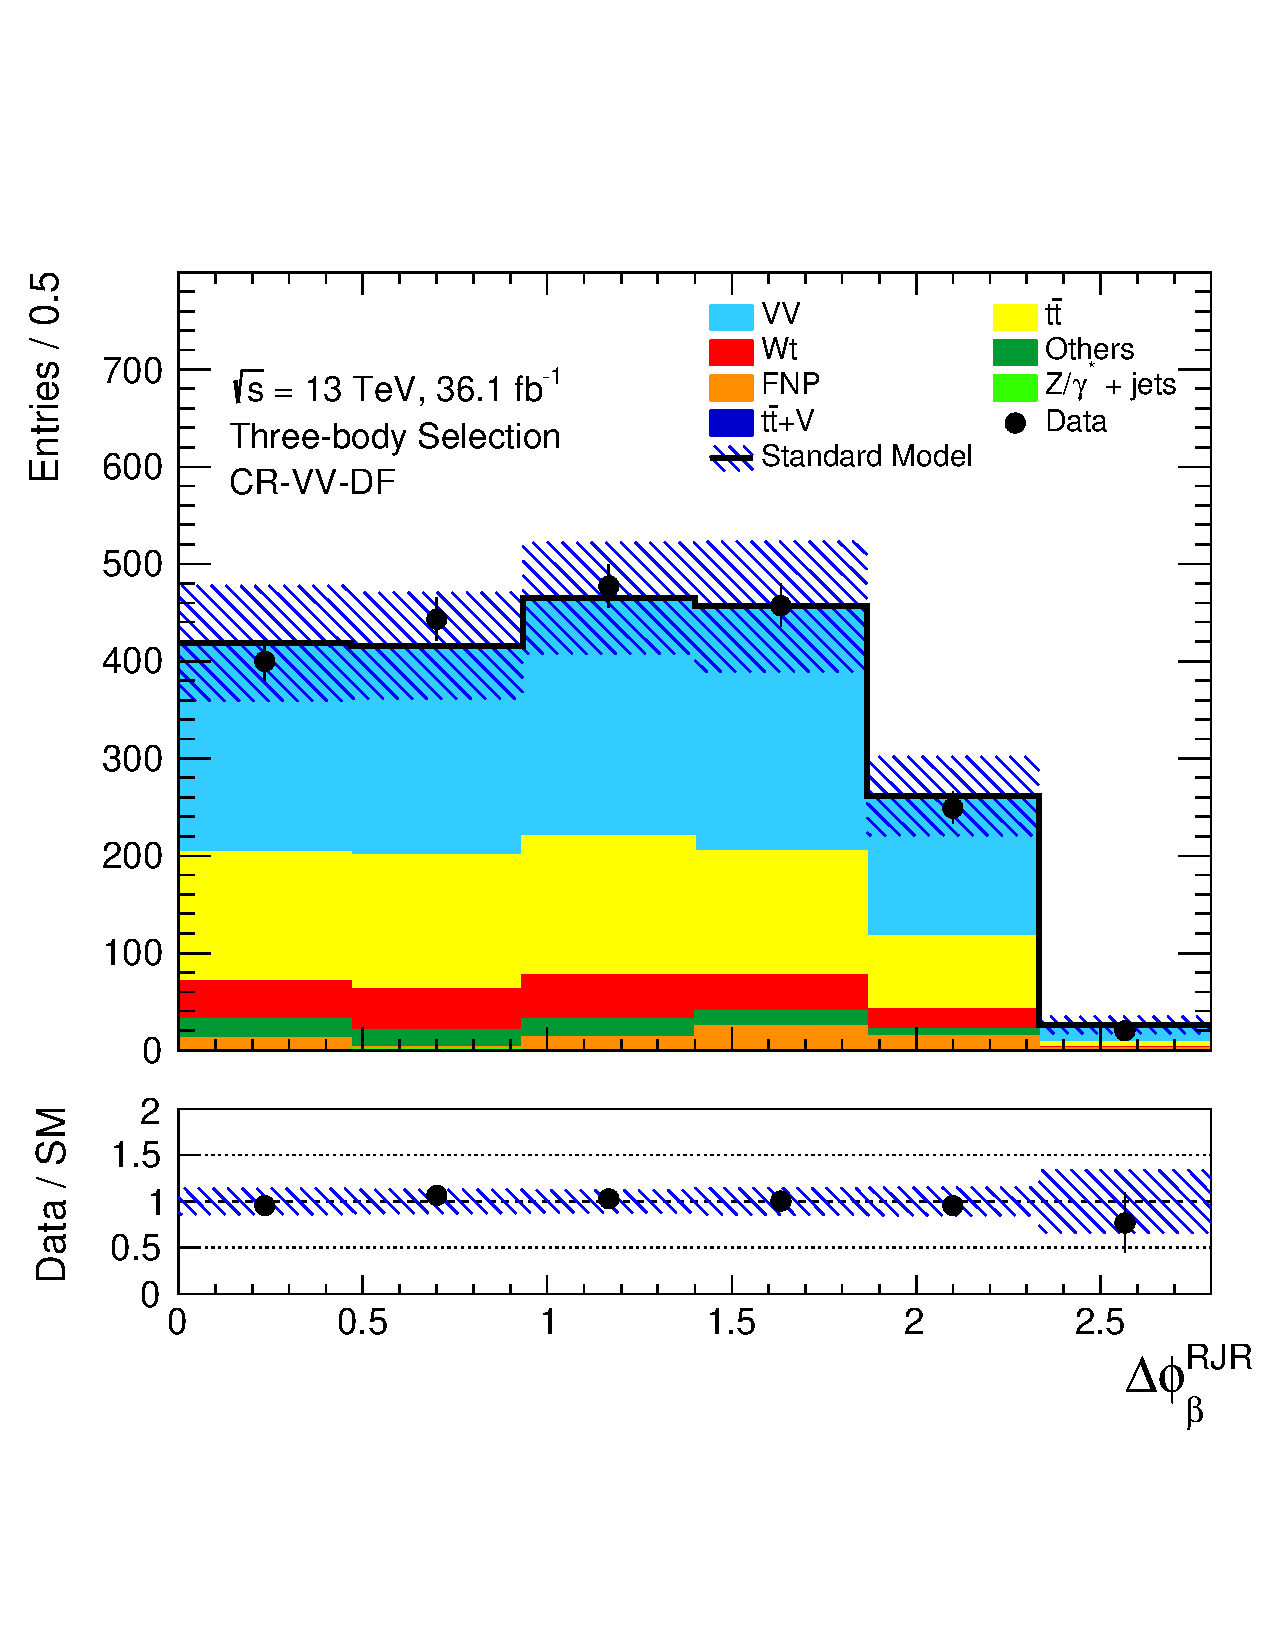
\includegraphics[width=0.48\textwidth]{figures/search_stop2l/bkg_est/crvdf/crv_DPB_vSS}
        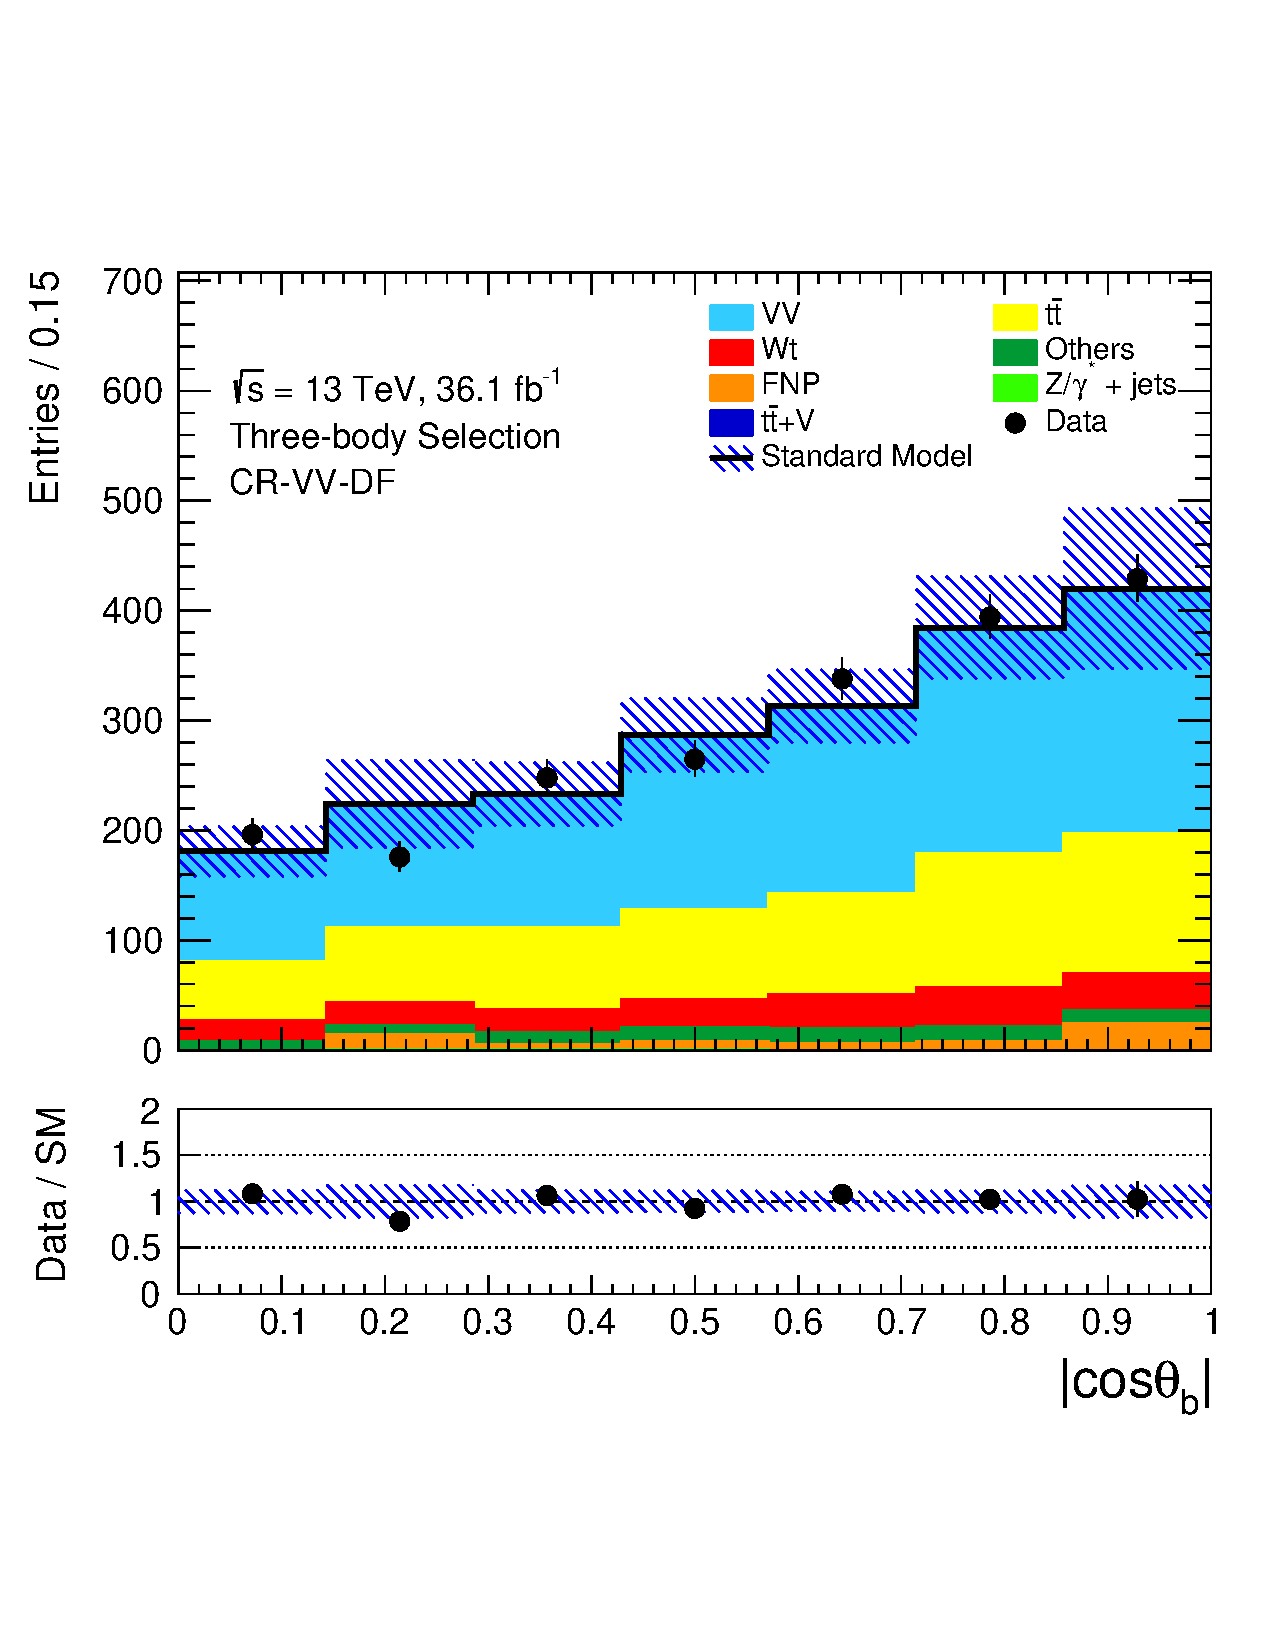
\includegraphics[width=0.48\textwidth]{figures/search_stop2l/bkg_est/crvdf/crv_cosThetaB}
        \caption{
            Distributions of \mdr (\textit{\textbf{upper left}}), leading lepton \pT~(\textit{\textbf{upper right}}),
            \dpb (\textit{\textbf{lower left}}), and $|\cosb|$ (\textit{\textbf{lower right}}) in the different-flavor diboson CR,
            CR-VV-DF.
            The error on the SM processes includes statistical and systematic uncertainties.
            The post-fit normalization correction factors for the \ttbar and diboson processes
            have been applied.
        }
        \label{fig:crvvDF_0}
    \end{center}
\end{figure}
\begin{figure}[!htb]
    \begin{center}
        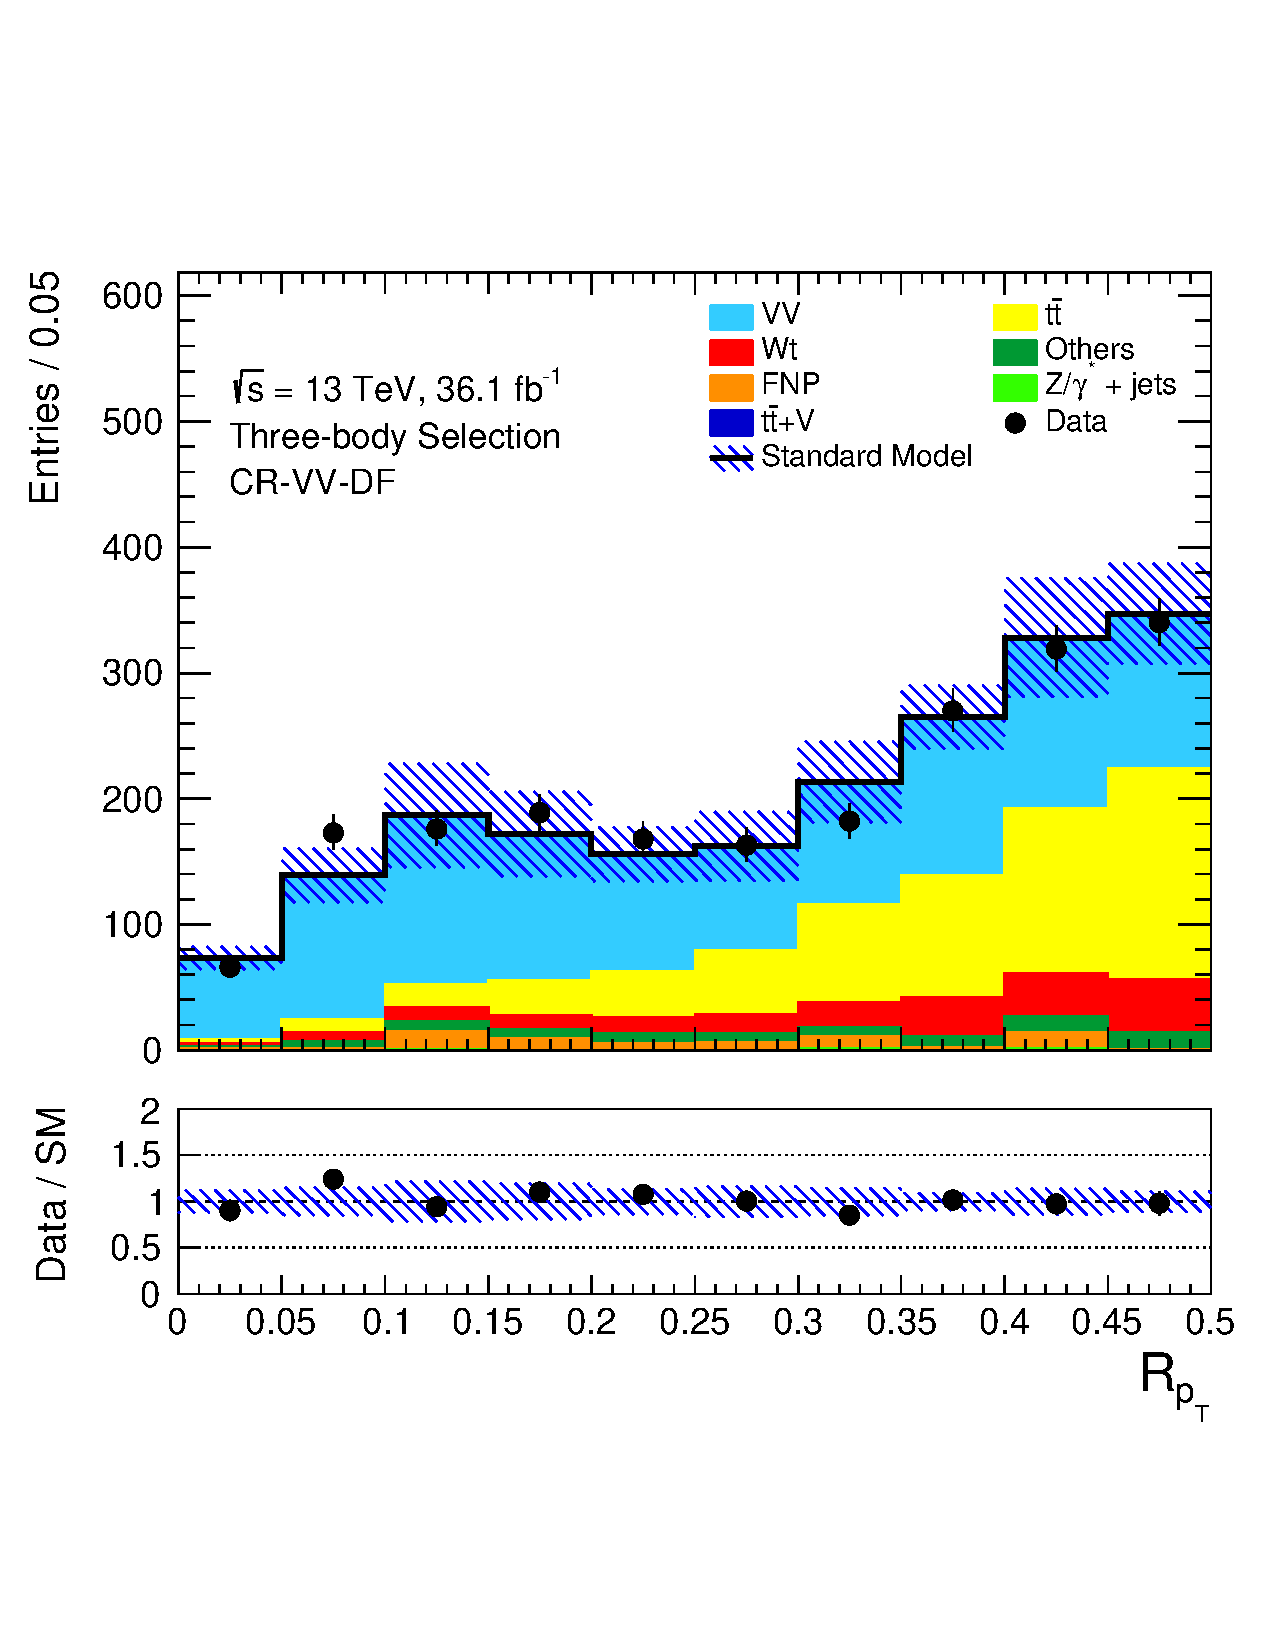
\includegraphics[width=0.48\textwidth]{figures/search_stop2l/bkg_est/crvdf/crv_RPT}
        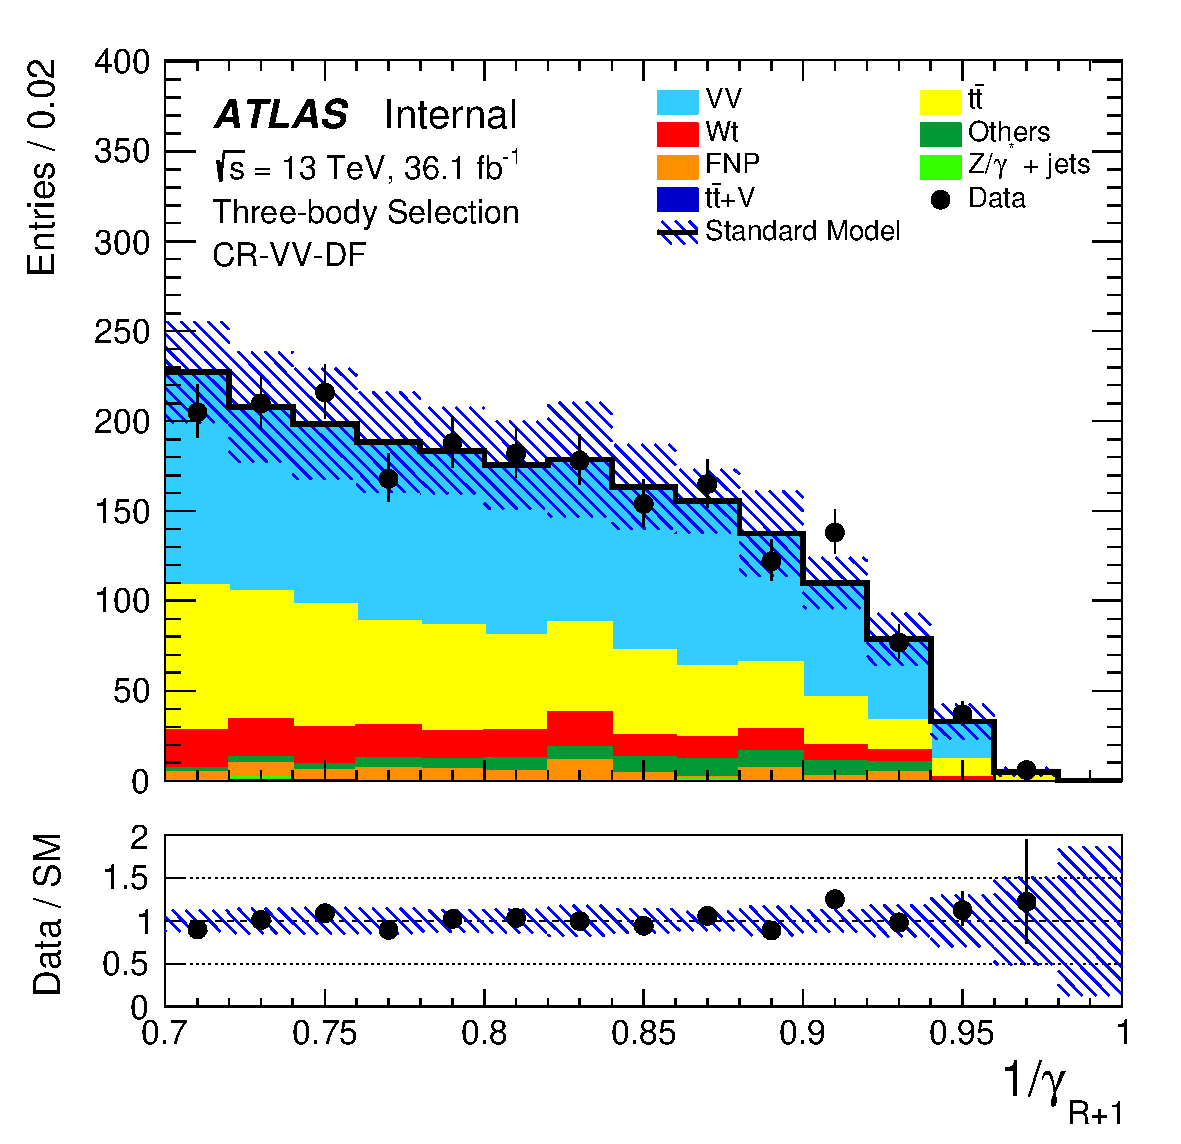
\includegraphics[width=0.48\textwidth]{figures/search_stop2l/bkg_est/crvdf/crv_gamInvRp1}
        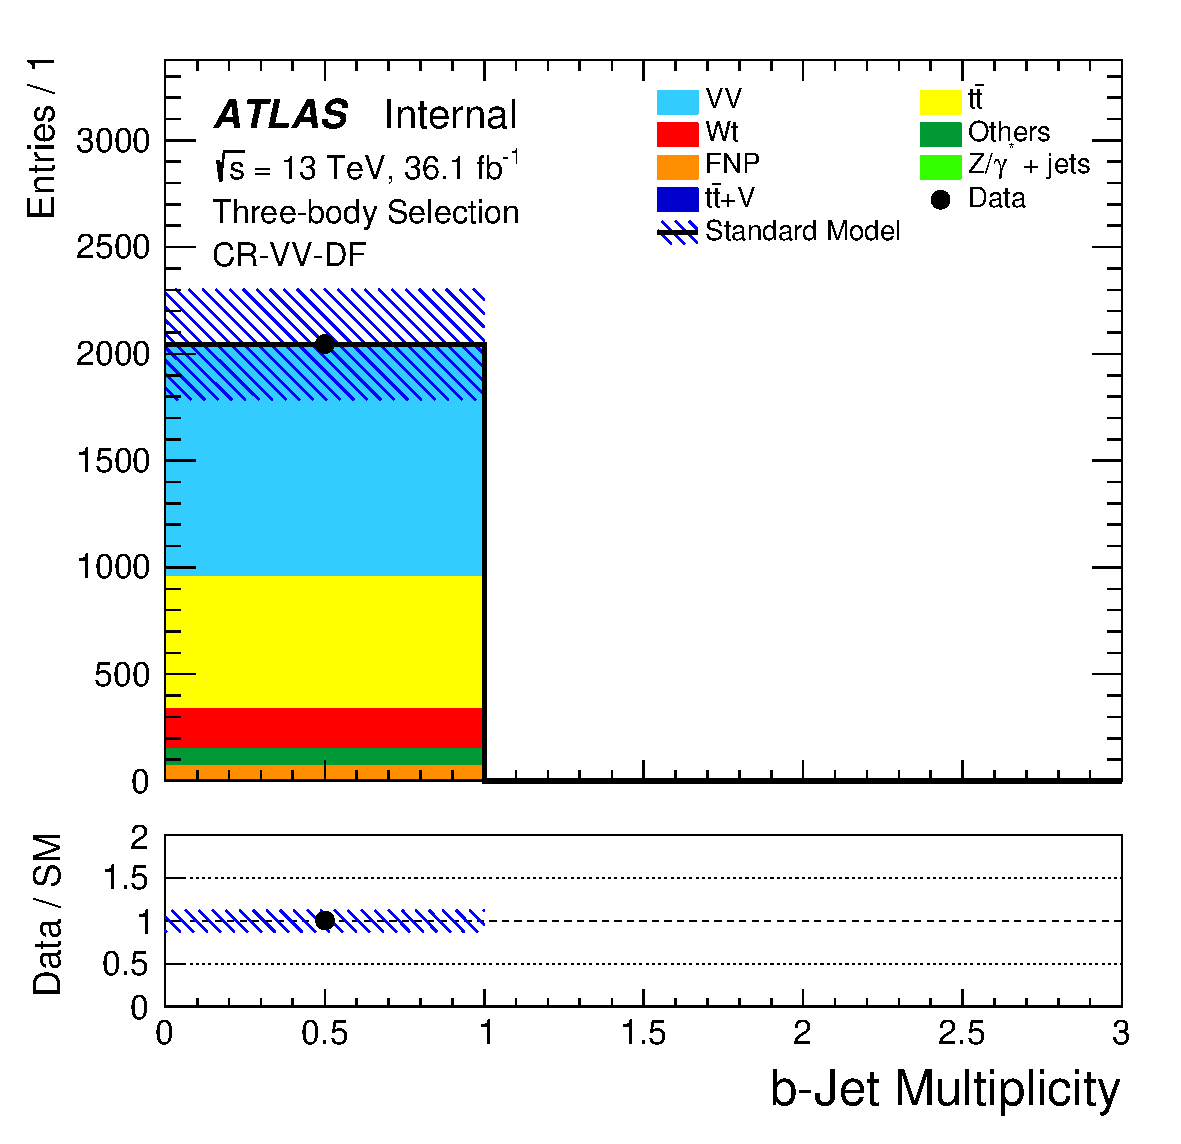
\includegraphics[width=0.48\textwidth]{figures/search_stop2l/bkg_est/crvdf/crv_nBJets}
        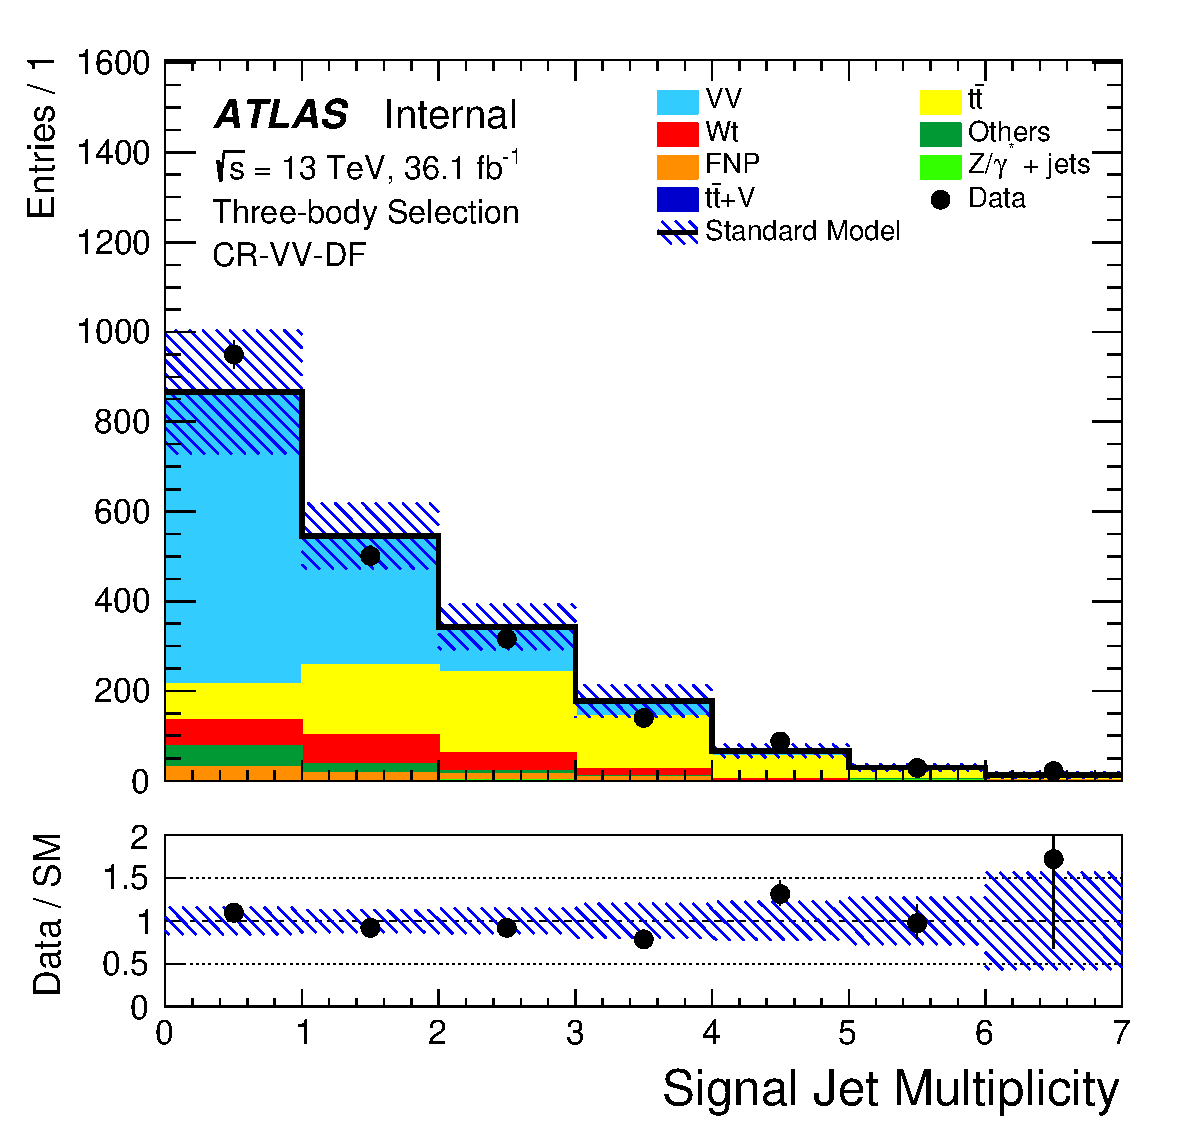
\includegraphics[width=0.48\textwidth]{figures/search_stop2l/bkg_est/crvdf/crv_nSJets}
        \caption{
            Distributions of \rpt (\textit{\textbf{upper left}}), leading lepton \gaminv~(\textit{\textbf{upper right}}),
            $b$-tagged jet multiplicity (\textit{\textbf{lower left}}), and non-$b$-tagged jet multiplicity(\textit{\textbf{lower right}}) in the different-flavor diboson CR,
            CR-VV-DF.
            The error on the SM processes includes statistical and systematic uncertainties.
            The post-fit normalization correction factors for the \ttbar and diboson processes
            have been applied.
        }
        \label{fig:crvvDF_1}
    \end{center}
\end{figure}

\FloatBarrier
%%%%%%%%%%%%%%%%%%%%%%%%%%%%%%%%%%%%%%%%%%%%%%%%%%%%%%%%%%%%%%%%%%%%%%%%%%%%%%%%%%%%%%%%%%%%
%%%%%%%%%%%%%%%%%%%%%%%%%%%%%%%%%%%%%%%%%%%%%%%%%%%%%%%%%%%%%%%%%%%%%%%%%%%%%%%%%%%%%%%%%%%%
%%%%%%%%%%%%%%%%%%%%%%%%%%%%%%%%%%%%%%%%%%%%%%%%%%%%%%%%%%%%%%%%%%%%%%%%%%%%%%%%%%%%%%%%%%%%
%
% POST FIT
%
%%%%%%%%%%%%%%%%%%%%%%%%%%%%%%%%%%%%%%%%%%%%%%%%%%%%%%%%%%%%%%%%%%%%%%%%%%%%%%%%%%%%%%%%%%%%
%%%%%%%%%%%%%%%%%%%%%%%%%%%%%%%%%%%%%%%%%%%%%%%%%%%%%%%%%%%%%%%%%%%%%%%%%%%%%%%%%%%%%%%%%%%%
%%%%%%%%%%%%%%%%%%%%%%%%%%%%%%%%%%%%%%%%%%%%%%%%%%%%%%%%%%%%%%%%%%%%%%%%%%%%%%%%%%%%%%%%%%%%

\subsection{Background-only Fit}
\label{sec:stop_background_only}

In order to assess the impact of the CRs on the background estimation in the SRs, a so-called `background-only'
fit is performed.
A background-only fit is profile-likelihood fit, as described Section~\ref{sec:likelihood},
in which the only regions contributing to the likelihood (c.f Equation~\ref{eq:full_likelihood})
are the analysis' CRs.
The result of running a background-only fit to data in the CRs is shown in Table~\ref{tab:bkgonly_CRVR},
which shows the MC predicted yields for the background processes both before and after the
background-only fit is performed, as well as the observed data counts, in each of the CRs and VRs in the analysis.
The post-fit yields in the CRs are expected to agree with the observed data counts, since the latter are used
as constraints in the fit model and there are as many freely-floating parameters in the fit (3 $\mu$ factors)
as there are CRs; therefore, the fit has enough freedom to cover any discrepancy between the observed data and pre-fit MC prediction of
the background processes.
The agreement observed between the post-fit MC and the observed data in the VRs shows that the extrapolation,
at least in terms of the corrected MC's normalisation, is performing well.

The normalisation correction factors for the \ttbar~and diboson processes obtained in the background-only
fit are listed in Table~\ref{tab:stop_scalefactors}.
They are generally consistent with one.

\begin{table}[!htb]
\begin{center}
\setlength{\tabcolsep}{0.0pc}
{\scriptsize
\caption{
Yields in the \ttbar~and diboson CRs and VRs for the \bWN search for the main background processes
contributing to the analysis.
The lower-portion of the table are the yields before the background-only fit to data
in the CRs, without the normalisation corrections applied.
The upper-portion of the table are those taken after the background-only fit to data.
The errors on the quoted numbers are due to the statistical and experimental systematic uncertainties.
}
\label{tab:bkgonly_CRVR}
\begin{tabular*}{\textwidth}{@{\extracolsep{\fill}}lrrrrrr}
\noalign{\smallskip}\hline\noalign{\smallskip}
\noalign{\smallskip}\hline\noalign{\smallskip}
\textbf{Process}           & \textbf{CR-Top}            & \textbf{CR-VV-DF}            & \textbf{CR-VV-SF}            & \textbf{VR-Top}           & \textbf{VR-VV-DF}            & \textbf{VR-VV-SF}              \\[-0.05cm]
\noalign{\smallskip}\hline\noalign{\smallskip}


Observed Data         & $951$              & $2046$              & $1275$              & $1197$              & $1896$              & $783$                    \\
\noalign{\smallskip}\hline\noalign{\smallskip}
%%
Post-fit Total SM         & $951.00 \pm 30.84$          & $2046.05 \pm 45.23$          & $1275.17 \pm 35.68$          & $1231.78 \pm 86.59$          & $2013.57 \pm 116.49$          & $780.44 \pm 117.32$              \\
\noalign{\smallskip}\hline\noalign{\smallskip}
%%
        Post-fit \ttbar          & $833.03 \pm 32.85$          & $619.74 \pm 111.40$          & $333.62 \pm 60.91$          & $733.87 \pm 64.91$          & $754.94 \pm 78.17$          & $127.14 \pm 22.09$              \\
%%
        Post-fit Diboson (DF)          & $11.51 \pm 2.43$          & $1093.28 \pm 125.83$          & $0.00 \pm 0.00$          & $331.13 \pm 82.57$          & $886.53 \pm 168.16$          & $0.00 \pm 0.00$              \\
%%
        Post-fit Diboson (SF)          & $0.00 \pm 0.00$          & $0.00 \pm 0.00$          & $378.94 \pm 124.32$          & $0.00 \pm 0.00$          & $0.00 \pm 0.00$          & $380.00 \pm 141.58$              \\
%%
        Post-fit Single-top          & $101.10 \pm 9.73$          & $186.47 \pm 27.99$          & $103.47 \pm 17.43$          & $111.52 \pm 14.49$          & $151.88 \pm 14.37$          & $36.40 \pm 5.62$              \\
%%
        Post-fit $\ttbar+V$          & $4.35 \pm 0.42$          & $0.39 \pm 0.07$          & $0.36 \pm 0.07$          & $1.27 \pm 0.22$          & $0.42 \pm 0.13$          & $0.05 \pm 0.02$              \\
%%
        Post-fit $Z$+jets          & $0.70 \pm 0.22$          & $1.83_{-1.83}^{+2.55}$          & $428.58 \pm 92.55$          & $0.47_{-0.47}^{+0.85}$          & $0.39_{-0.39}^{+0.71}$          & $191.37 \pm 78.38$              \\
%%
        Post-fit Single-higgs          & $0.31 \pm 0.13$          & $78.95 \pm 9.17$          & $6.23 \pm 1.06$          & $0.44_{-0.44}^{+0.52}$          & $54.98 \pm 4.34$          & $9.40 \pm 1.11$              \\
%%
        Post-fit Fakes          & $0.00 \pm 0.00$          & $65.37 \pm 2.22$          & $23.96 \pm 1.25$          & $53.09 \pm 1.92$          & $164.42 \pm 5.68$          & $36.09 \pm 3.04$              \\
%%
 \noalign{\smallskip}\hline\noalign{\smallskip}
%%
 Total SM               & $905.14 \pm 16.54$          & $1988.38 \pm 110.43$          & $1248.21 \pm 123.42$          & $1184.39 \pm 71.23$          & $1952.92 \pm 61.72$          & $764.65 \pm 99.06$              \\
\noalign{\smallskip}\hline\noalign{\smallskip}
%%
         \ttbar          & $787.43 \pm 11.29$          & $585.87 \pm 102.00$          & $315.39 \pm 55.87$          & $693.71 \pm 53.51$          & $713.64 \pm 66.57$          & $120.19 \pm 20.17$              \\
%%
         Diboson (DF)          & $11.25 \pm 1.62$          & $1069.46 \pm 12.45$          & $0.00 \pm 0.00$          & $323.89 \pm 50.27$          & $867.18 \pm 77.75$          & $0.00 \pm 0.00$              \\
%%
         Diboson (SF)          & $0.00 \pm 0.00$          & $0.00 \pm 0.00$          & $370.13 \pm 15.48$          & $0.00 \pm 0.00$          & $0.00 \pm 0.00$          & $371.16 \pm 34.38$              \\
%%
         Single-top          & $101.10 \pm 9.80$          & $186.49 \pm 28.25$          & $103.49 \pm 17.59$          & $111.52 \pm 14.60$          & $151.88 \pm 14.46$          & $36.41 \pm 5.66$              \\
%%
         $\ttbar+V$          & $4.35 \pm 0.42$          & $0.39 \pm 0.07$          & $0.36 \pm 0.07$          & $1.27 \pm 0.23$          & $0.42 \pm 0.13$          & $0.05 \pm 0.02$              \\
%%
         $Z$+jets          & $0.70 \pm 0.23$          & $1.83_{-1.83}^{+2.57}$          & $428.65 \pm 93.15$          & $0.48_{-0.48}^{+0.86}$          & $0.40_{-0.40}^{+0.72}$          & $191.36 \pm 78.78$              \\
%%
         Single-higgs          & $0.31 \pm 0.13$          & $78.96 \pm 9.26$          & $6.23 \pm 1.07$          & $0.44_{-0.44}^{+0.53}$          & $54.98 \pm 4.37$          & $9.40 \pm 1.12$              \\
%%
         Fakes          & $0.00 \pm 0.00$          & $65.37 \pm 2.23$          & $23.96 \pm 1.26$          & $53.09 \pm 1.92$          & $164.42 \pm 5.70$          & $36.09 \pm 3.04$              \\
\noalign{\smallskip}\hline\noalign{\smallskip}
\noalign{\smallskip}\hline\noalign{\smallskip}
\end{tabular*}
}
\end{center}
\end{table}

\begin{table}[!htb]
    \begin{center}
        \caption{
            Normalisation correction factors for the \ttbar~$(\mu_{\ttbar})$,
            same-flavor diboson $(\mu_{\text{VV-SF}})$, and different-flavor diboson $(\mu_{\text{VV-DF}})$
            processes derived from the background-only fit to the CRs.
            The errors on the quoted numbers are due to the statistical and experimental systematic uncertainties
            entering the fit.
        }
        \label{tab:stop_scalefactors}
        \begin{tabular}{l|c}
            \hline
            \hline
                $\mu_{\ttbar}$ & $1.06 \pm 0.05$ \\
                $\mu_{\text{VV-SF}}$ & $1.02 \pm 0.35$ \\
                $\mu_{\text{VV-DF}}$ & $1.02 \pm 0.12$ \\
            \hline
            \hline
        \end{tabular}
    \end{center}
\end{table}

